%TODO:
%   Experiments - Feas % x tf x cvs 
%		Add figure to illustrate online schedule with auto update HVAC
%		Add more experiments of online?  ---- impact of cvs and tf in online scenario 
%		Add online scheduling literature
%		Add stochastics as future or ??

%   The model should be able to handle impromptu scheduling request and response in time in an \emph{online} manner.

\chapter{Handling Online Requests}
\label{cha:online}

\section{Introduction}

In Chapter \ref{cha:lns}, we presented a scalable joint HVAC control and occupancy scheduling model by combining MIP and LNS. Within a short computational time, this model is capable of minimising HVAC utilisation by scheduling an extensive number of group activities to take place at a large number of building zones and time slots.
However, this approach was offline and assumes all activities to schedule and other parameters such as the weather forecast and solar gains are known in advance. Although the model generates energy-efficient schedules, its practicability is nevertheless limited in the real-world. In reality, scheduling requests can arrive at any time of the day using existing room booking systems. 
In a recent survey, \cite{kwak2013tesla} shows that 56\% of meeting requests were made within one day before the actual meeting day. Thus, the ability to handle dynamically arriving requests is crucial. Moreover, the ability to update HVAC control following a change in weather forecast is also important. 

In this chapter, we extend the HVAC-aware occupancy scheduling approach to process activity requests in an \textsl{online} manner. In more detail, we present an online approach that models and solves the joint HVAC control and occupancy scheduling problem. The model needs to be responsive to dynamic information such as new activity requests and weather updates. Our online algorithm greedily commits to the best schedule for the latest activity requests and notifies the occupants immediately, but revises the entire future HVAC control strategy each time it considers new requests and weather updates. This allows the integrated model to handle incoming requests in a prompt manner whilst continuously optimising the HVAC control reflecting updated weather forecast and activity schedules. In our experiments, the quality of the solution obtained by this approach is within 1\% of that of the clairvoyant solution. 

In the next section, we show how our integrated model is being transformed into an online model. We further elaborate on how the online model is scaled with the LNS method. In Section \ref{sec:online:experiments} we compare our model with the clairvoyant solution, showing the efficacy of this simple and effective online algorithm. We discuss about related work in Section \ref{sec:online:related_work}. We then conclude the chapter %and discuss potential future works 
in Section \ref{sec:online:conclusion}.


\section{Online HVAC-Aware Occupancy Scheduling} \label{sec:online:sche_model}

This section presents our online occupancy scheduling and HVAC control problem. We start by describing the online setting and our notations. We then cover the scheduling constraints and variables which, later on, will interact with the HVAC control model to form the complex joint scheduling and control model. Following our work from the previous chapters, we formulate our model as a MIP. It can be solved using a MIP solver, or when scaling up to problems of practical size, by combining MIP with LNS.

In our online setting, the scheduler runs recurrently and each run is called an \emph{online session}. Each online session $i\in I$ starts at time $\tau_i$ and ends before the next session starts at time $\tau_{i+1}$. The scheduling and control model discretizes time into a set $K$ of {\em time steps}. Each time step $k\in K$ starts at time $t_{k}$. Two consecutive time steps $k$ and $k+1$ are separated by a fixed duration $t_{k+1}-t_{k} = \bm{\Delta_t} \in \mathbb{R}^+$. Each online session $i$ considers a horizon of $\bm{n}$ time steps $K(i) = \{k(i), \ldots, k(i)+\bm{n}-1\}$ where $k(i)$, the first time step in that horizon, is the least time step in $K$ such that $t_{k(i)} \geq \tau_i$. 

\subsection{Scheduling Model}
Let $L$ be the set of locations (or, interchangeably, zones) in the building, and $P$ be a set of participants. An activity request $m$ is a tuple $\langle \bm{a}_m, K_m, L_m, P_m, \bm{d}_m \rangle$ where $\bm{a}_m \in \mathbb{R}^{+}$ is the request arrival time, $K_m\subseteq K$ is the set of time steps at which the activity is permitted to \underline{start} in the future (for each $k\in K_m, \bm{a}_m < t_k$), $L_m\subseteq L$ is the set of locations at which the activity is permitted to take place, $P_m\subseteq P$ is the set of attendees for the activity and $\bm{d}_m \in \mathbb{N}$ is the activity duration (number of time steps). As in the previous chapter, note that the sets $K_m$ and $L_m$ can be used to encode a variety of situations, such as room capacity requirements, availability of special equipment such as video conferencing, time deadlines for the activity, and attendee availability constraints. We write ${\cal C}(M)$ for the set of attendee conflicts w.r.t. a set of requests $M$; each conflict $C$ is a subset of requests, each pair of which has at least one attendee in common: ${\cal C}(M)=\{C\subseteq M \mid \forall m,m'\in C, P_m\cap P_{m'} \neq \emptyset \}$.

To account for all activities that have been scheduled so far, we maintain a master schedule $S$ as a set of triples $\langle m, l,k \rangle$ storing the activity request id $m$, the assigned location $l$, and the time step $k$ at which $m$ is scheduled to start. 
At each online session $i$, the scheduler schedules the new activity requests $N(i)$ which have been received since the start of session $i-1$, i.e, each $m\in N(i)$ satisfies $\tau_{i-1} < \bm{a}_m \leq \tau_{i}$. It also needs to consider, without modifying them, the set $Q(i)$ of ongoing activities and future activities that were scheduled during previous sessions: $Q(i) =\{m \mid \exists \langle m,l,k \rangle \in S\mbox{~such that~} k +\bm{d}_m -1 \geq k(i)\}$.
So overall, the set of activities to consider at session $i$ is $M(i) = N(i) \cup Q(i)$. To simplify the scheduling model below, we assume that for each pre-scheduled request $m \in Q(i)$ such that $\langle m,l,k \rangle \in S$, the set of permissible locations is reduced to $L_m =\{l\}$, and the set of permissible start time steps is reduced to the scheduled start time $k$ or the first time step $k(i)$ of the session, which ever occurs last, i.e. $K_m = \{\max(k,k(i))\}$. For consistency, the meeting duration $\bm{d}_m$ is decremented by $k(i)-k$.

\begin{figure}[t]
\centering
\includegraphics[width=5in,keepaspectratio]{figs/timeline.jpg}	
\caption{Online scenario}
\label{fig:timeline}
\end{figure}

Fig.~\ref{fig:timeline} shows a scenario example featuring three requests $m_1, m_2$ and $m_3$ with arrival times $\bm{a}_1$, $\bm{a}_2$ and $\bm{a}_3$, respectively. The set of locations is $L=\{{\bm l}_1,{\bm l}_2\}$. The dash vertical lines show the start of the sessions, and the dotted vertical lines delimit the time steps. In this instance, the scheduler runs every 10 minutes and the time steps are 30 minutes long. At the start of session $i=302$, requests $m_1$ and $m_2$ have already been scheduled and $m_3$ is a new request,
hence $N(302) = \{m_3\}$, $Q(302) = \{m_1,m_2\}$. The master schedule is $S=\{\langle m_1, {\bm l}_1, 102\rangle, \langle m_2, {\bm l}_1, 100\rangle\}$, and the first time step of the new session is $k(302) = 101$. The set of permissible locations and start time steps for the new request are $K_3=\{101,102\}$ and $L_3=\{{\bm l}_1,{\bm l}_2\}$ (${\bm l}_1$ will be ruled out by the scheduler).
Those of the pre-existing requests are reduced as follows: $L_1 =\{{\bm l}_1\}, K_1=\{102\}, L_2 = \{{\bm l}_1\}$ and $K_2 =\{101\}$. 

We are now ready to describe our scheduling constraints and variables for online session $i$. Similarly, as defined in the previous chapter, the main scheduling variable is the boolean decision variable $x_{m,l,k}$ which is true iff request $m\in M(i)$ is scheduled to take place at zone $l\in L_m$ starting at time slot $k\in K_m$. We also introduce the variables $y_{m,l,k}$ which is true iff activity $m$ is scheduled to occupy location $l$ at time step $k$, $z_{l,k}$ which is true iff zone $l$ is occupied at time step $k$, and $pp_{l,k}$ which indicates the number of people in zone $l$ at time step $k$. These variables will be used by the HVAC control part of the model in Section \ref{sec:online_hvac_model}.

%The scheduling constraints are similar to the model presented in chapter \ref{cha:milp}, with an exception that the scheduling horizon $k$ changes for each online session $i$. 
Constraints \eqref{eq:online_ms_everytype} ensure that all requests are scheduled exactly once within the allowable start times and locations. $\psi_m$ represents the number of meetings of type $m$ with similar time windows, the same number of attendees, and the same attendee conflicts.
Constraints \eqref{eq:online_ms_y} define the $y_{m,l,k}$ variables. Constraints \eqref{eq:online_ms_totalalloc} state that no more than one activity can occupy a location at any time and define the $z_{l,k}$ variables. 
Constraints \eqref{eq:online_ms_totalnum} determine the number ${pp}_{l,k}$ of occupants at each location and time step, and finally constraints \eqref{eq:online_ms_meeting} ensure that activities with at least one attendee in common cannot be scheduled in parallel. 
Once a new request $m\in N(i)$ has been scheduled, the master schedule $S$ is updated by adding the 3-tuple $\langle m,l,k\rangle$ for which $x_{m,l,k} =1$.

\begin{align}
\mathop{\sum \limits_{l\in L_m, k \in K_m}} \hspace{-12pt} x_{m,l,k} &= \psi_m \hspace{10pt} \forall m \in M(i)  \label{eq:online_ms_everytype}  \\
%\mathop{\sum \limits_{l\in L_m, k \in K_m}} \hspace{-12pt} x_{m,l,k} &= 1 \hspace{10pt} \forall m \in M(i) \label{eq:online_ms_every} \\
\mathop{\sum \limits_{\substack{k' \in K_m: \\
l\in L_m, \hspace{5pt} k-\bm{d}_m+1 \leq k' \leq k}}} \hspace{-12pt} x_{m,l,k'} & = y_{m,l,k} \hspace{10pt} \forall m \in M(i), l \in L, k \in K(i) \label{eq:online_ms_y} \\
\mathop{\sum \limits_{m \in M(i)}} \hspace{5pt} y_{m,l,k} &\leq z_{l,k} \hspace{10pt} \forall l \in L, k \in K(i) \label{eq:online_ms_totalalloc} \\
\mathop{\sum \limits_{m \in M(i)}} y_{m,l,k}\times \left| P_m\right| &= {pp}_{l,k} \hspace{10pt} \forall l \in L, k \in K(i) \label{eq:online_ms_totalnum} \\
\mathop{\sum \limits_{m \in \nu,l \in L_m}} y_{m,l,k} &\leq 1 \hspace{10pt} \forall k \in K(i), \nu \in {\cal C}(M(i)) \label{eq:online_ms_meeting}
\end{align}

%Note that to simplify the model, the scheduling constraints for all ongoing activities and future activities $m \in Q(i)$ that were scheduled during previous sessions can be omitted. We may remove constraints \eqref{eq:online_ms_everytype}-\eqref{eq:online_ms_y} for these meetings and set \eqref{eq:online_ms_totalalloc} and \eqref{eq:online_ms_totalnum} to
%\begin{align}
%z_{l,k} &= 1 \hspace{10pt} \forall m \in Q(i), l \in L_m, k \in K^o_m \label{eq:ms_totalalloc_occ} \\
%\left| P_m\right| &= {pp}_{l,k} \hspace{10pt} \forall m \in Q(i), l \in L_m, k \in K^o_m  \label{eq:ms_totalnum_occ}.
%\end{align}
%\noindent where $K^o_m = \left\{K^o_m \subseteq K | \forall k \in K^o_m, m \in Q(i), l \in L_m, x_{m,l,k'} = 1, k = \left\{k'\!,\!k'+1\!,\! \ldots\!,k'\!+\!d_m\!-\!1\right\} \right\}$. Note that Constraints \eqref{eq:online_ms_meeting} can also be omitted for pre-scheduled meetings. This is achieved by removing all slots that are pre-occupied by the conflicting attendees. %while generating $\nu \in {\cal C}(M(i))$ for new meetings. 
%These steps greatly reduced the number of variables and constraints, avoiding unnecessary search in MIP.
  
\subsection{HVAC Control Model} \label{sec:online_hvac_model}

The HVAC control model is similar to the model presented in Chapter \ref{cha:milp}, with an exception that the scheduling horizon $k$ changes for each online session $i$. We use the reduced model which considers only external walls in Equation \eqref{eq:roomtemperature_lns}. Our goal is to generate energy-efficient schedules that minimise the energy use of air-conditioning, re-heating and fan operations of the HVAC, considering all on-going, future and new meetings known upon the online session $i$ starts. Thus, similar to before, the objective function for each session $i$ is the following.

\begin{equation} 
\mbox{minimise} \sum_{k\in K(i)}  \left( p_{k}^{cond} + p_{k}^{fan} + \sum_{l \in L} p_{l,k}^{heat}\right) \times \bm{\Delta_t}
\end{equation}
where
\begin{align}
p_{k}^{fan} &= \bm{\beta} \sum_{l \in L} a_{l,k}^{SA} \quad  \forall k \in K(i) \label{eq:online:p_fan} \\
p_{k}^{cond} &= \bm{C^{pa}}\left(\bm{T_{k}^{OA}}(i) - \bm{T^{CA}}\right) \sum_{l \in L}  a_{l,k}^{SA} \quad \forall k \in K(i) \label{eq:online:p_cond} \\
p_{l,k}^{heat} &= \bm{C^{pa}} (T_{l,k}^{SA}- \bm{T^{CA}}) a_{l,k}^{SA} \quad \forall l \in L,k \in K(i) \label{eq:online:p_heat}
\end{align}

In Constraints~(\ref{eq:online:p_cond}), we assume that online session $i$ uses the latest update $T_{k}^{OA}(i)$ available for the outdoor temperature forecast at each time step $k$. 
The temperature at each zone and time step, and the effects of the HVAC control on this zone temperature is constrained by \eqref{eq:online:comfort}-\eqref{eq:online:aSA_bound}

\begin{align}
\undersl{\bm{T}}^{\emptyset} + \undersl{\bm{T}}^gz_{l,k} &\leq T_{l,k} \leq \oversl{\bm{T}}^{\emptyset} - \oversl{\bm{T}}^gz_{l,k} \quad \forall l\in L , k \in K(i) \label{eq:online:comfort} \\
\bm{T}^{CA} \leq T^{SA}_{l,k} &\leq \oversl{\bm{T}}^{SA} \quad \forall l \in L, k \in K(i) \label{eq:online:TSA_bound} \\
\undersl{\bm a}^{SA} \leq a^{SA}_{l,k} &\leq \oversl{\bm a}^{SA} \quad \forall l \in L, k \in K(i) \label{eq:online:aSA_bound}
\end{align}

The zone thermal dynamics is updated following the discrete-time linear model in Chapter \ref{cha:milp}, but we use the latest available forecast of the solar gain $Q^s_{l,k}(i)$and outdoor temperature $T_{k}^{OA}(i)$. 
\begin{align}
T_{l,k+1} = f_{l}(T_{l,k}, u_{l,k}, v_{l,k}) \quad \forall l \in L, k \in K(i) 
\end{align}  
where $u_{l,k} = [a^{SA}_{l,k}, T^{SA}_{l,k},pp_{l,k}]$ is the vector of controllable variables, and $v_{l,k} = [\bm{Q^s_{l,k}}(i), \\\bm{T^{OA}_k}(i)]$ is the vector of exogenous inputs. Given that $z_{l,k}$ links the scheduling model with the zone thermal dynamics model, the HVAC control is optimised over the entire horizon $K(i)$. For example, the HVAC control could be revised in each locations upon receiving new meetings, updated weather information and solar gains in each online session.


\subsection{Online LNS}

To solve this online model, we reformulate our MIP model with Large Neighborhood Search explained in Chapter \ref{cha:lns}. In brief, our online LNS approach works as outlined in Algorithm \ref{alg:online:lns}.

\begin{algorithm}[ht!]
\small
%\SetAlgoLined
\SetKwFunction{Return}{return}
\SetKwInput{Input}{Input}
\SetKwInput{Output}{Output}
\SetKwInput{Initialize}{Initialization}
\SetKwInput{Algorithm}{Destroy \& Repair}
\SetKwIF{If}{ElseIf}{Else}{if}{then}{else if}{else}{endif}
 \Indm
 \Input{Ongoing \& new requests $M(i)=Q(i) \cup N(i)$, Rooms $L$, time steps $K(i)$}
 \Output{Master Schedule $S$ }
 \Initialize{}
 \Indp{$S(i) \gets \emph{GenInitialMeetingSchedule}(M(i), K(i), L)$\\
$ J \gets \emph{GenHVACControl}(S(i))$
 }\;
 \Indm
 \Algorithm{}
 \Indp
 \While{not LnsTimeUp()}
 {
	$L' \gets \emph{SelectNeighborhood}\left(L\right)$ \\
	$\emph{DestroyNeighborhood}\left(S(i), N(i), L' \right)$ \\
	$\langle S'(i), J' \rangle \gets \emph{RepairNeighborhood}\left(S(i), N(i), L' \right)$\\
	\If{$J' < J$}	
	{
		$J \gets J' $\\
		$\emph{UpdateSchedule}\left(S'(i), S(i) \right)$
	}
 }
 \Return $S$
 \caption{LNS approach in each online session $i$}
 \label{alg:online:lns}
\end{algorithm}

In every online session $i$, we start by generating an initial feasible solution, in two steps. First, we find a feasible occupancy schedule that minimises the number of rooms used. Second, we determine the HVAC control settings (supply air flow rate and temperature) that minimise energy consumption for this schedule.

Our destroy step destroys part of the schedule by unscheduling the subset of new requests $N(i)$ that are allocated to two to four randomly selected locations. This forms an energy-aware meeting scheduling subproblem that is much smaller than the original problem and can be solved effectively using MIP. The repair step consists in repairing the schedule and re-optimising the entire HVAC control by solving this subproblem using our MIP model. If this leads to an improved solution, then the new schedule and control settings are accepted. Otherwise, we keep the solution that was just destroyed. Given that the LNS always start with a feasible solution, the solution remains feasible throughout the execution of the algorithm.


\subsection{Scenario Example}


%\begin{sidewaysfigure}[h]
    %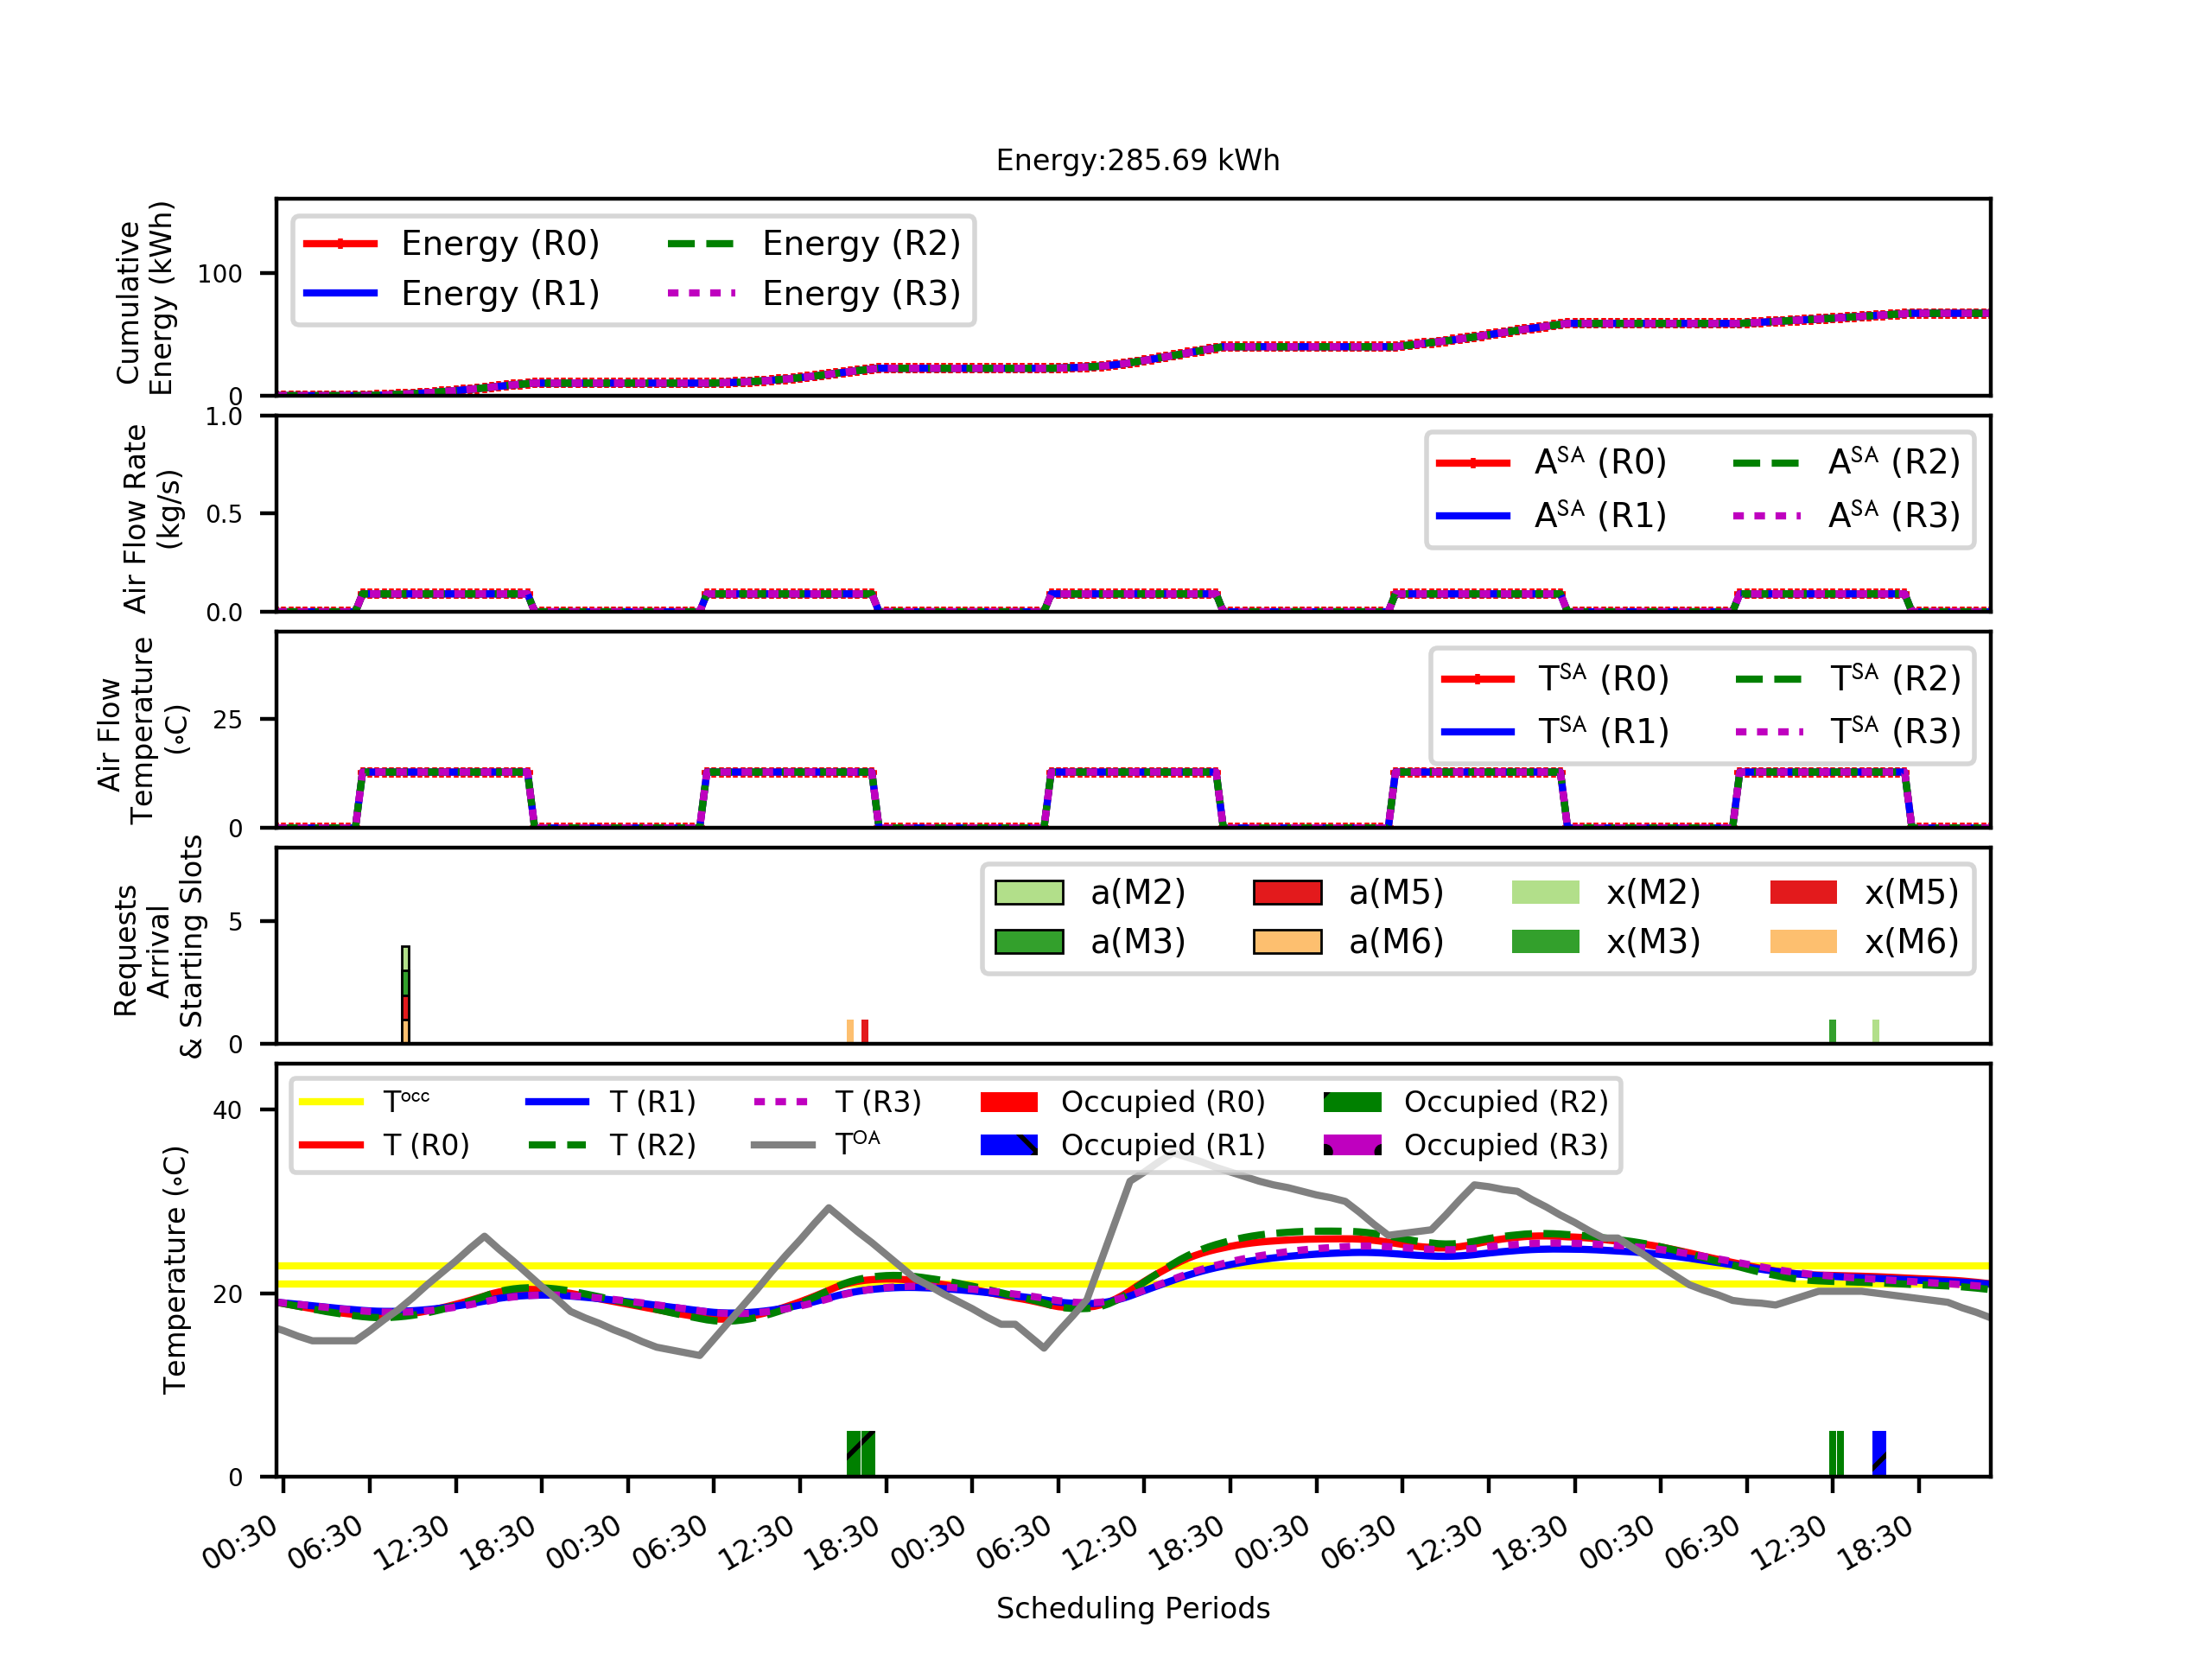
\includegraphics[width=0.9\linewidth]{figs/online_r0.png}
    %\caption{Online Scheduling - Session 1}
    %\label{fig:online_eg1}
%\end{sidewaysfigure}
%
%\begin{sidewaysfigure}[h]
    %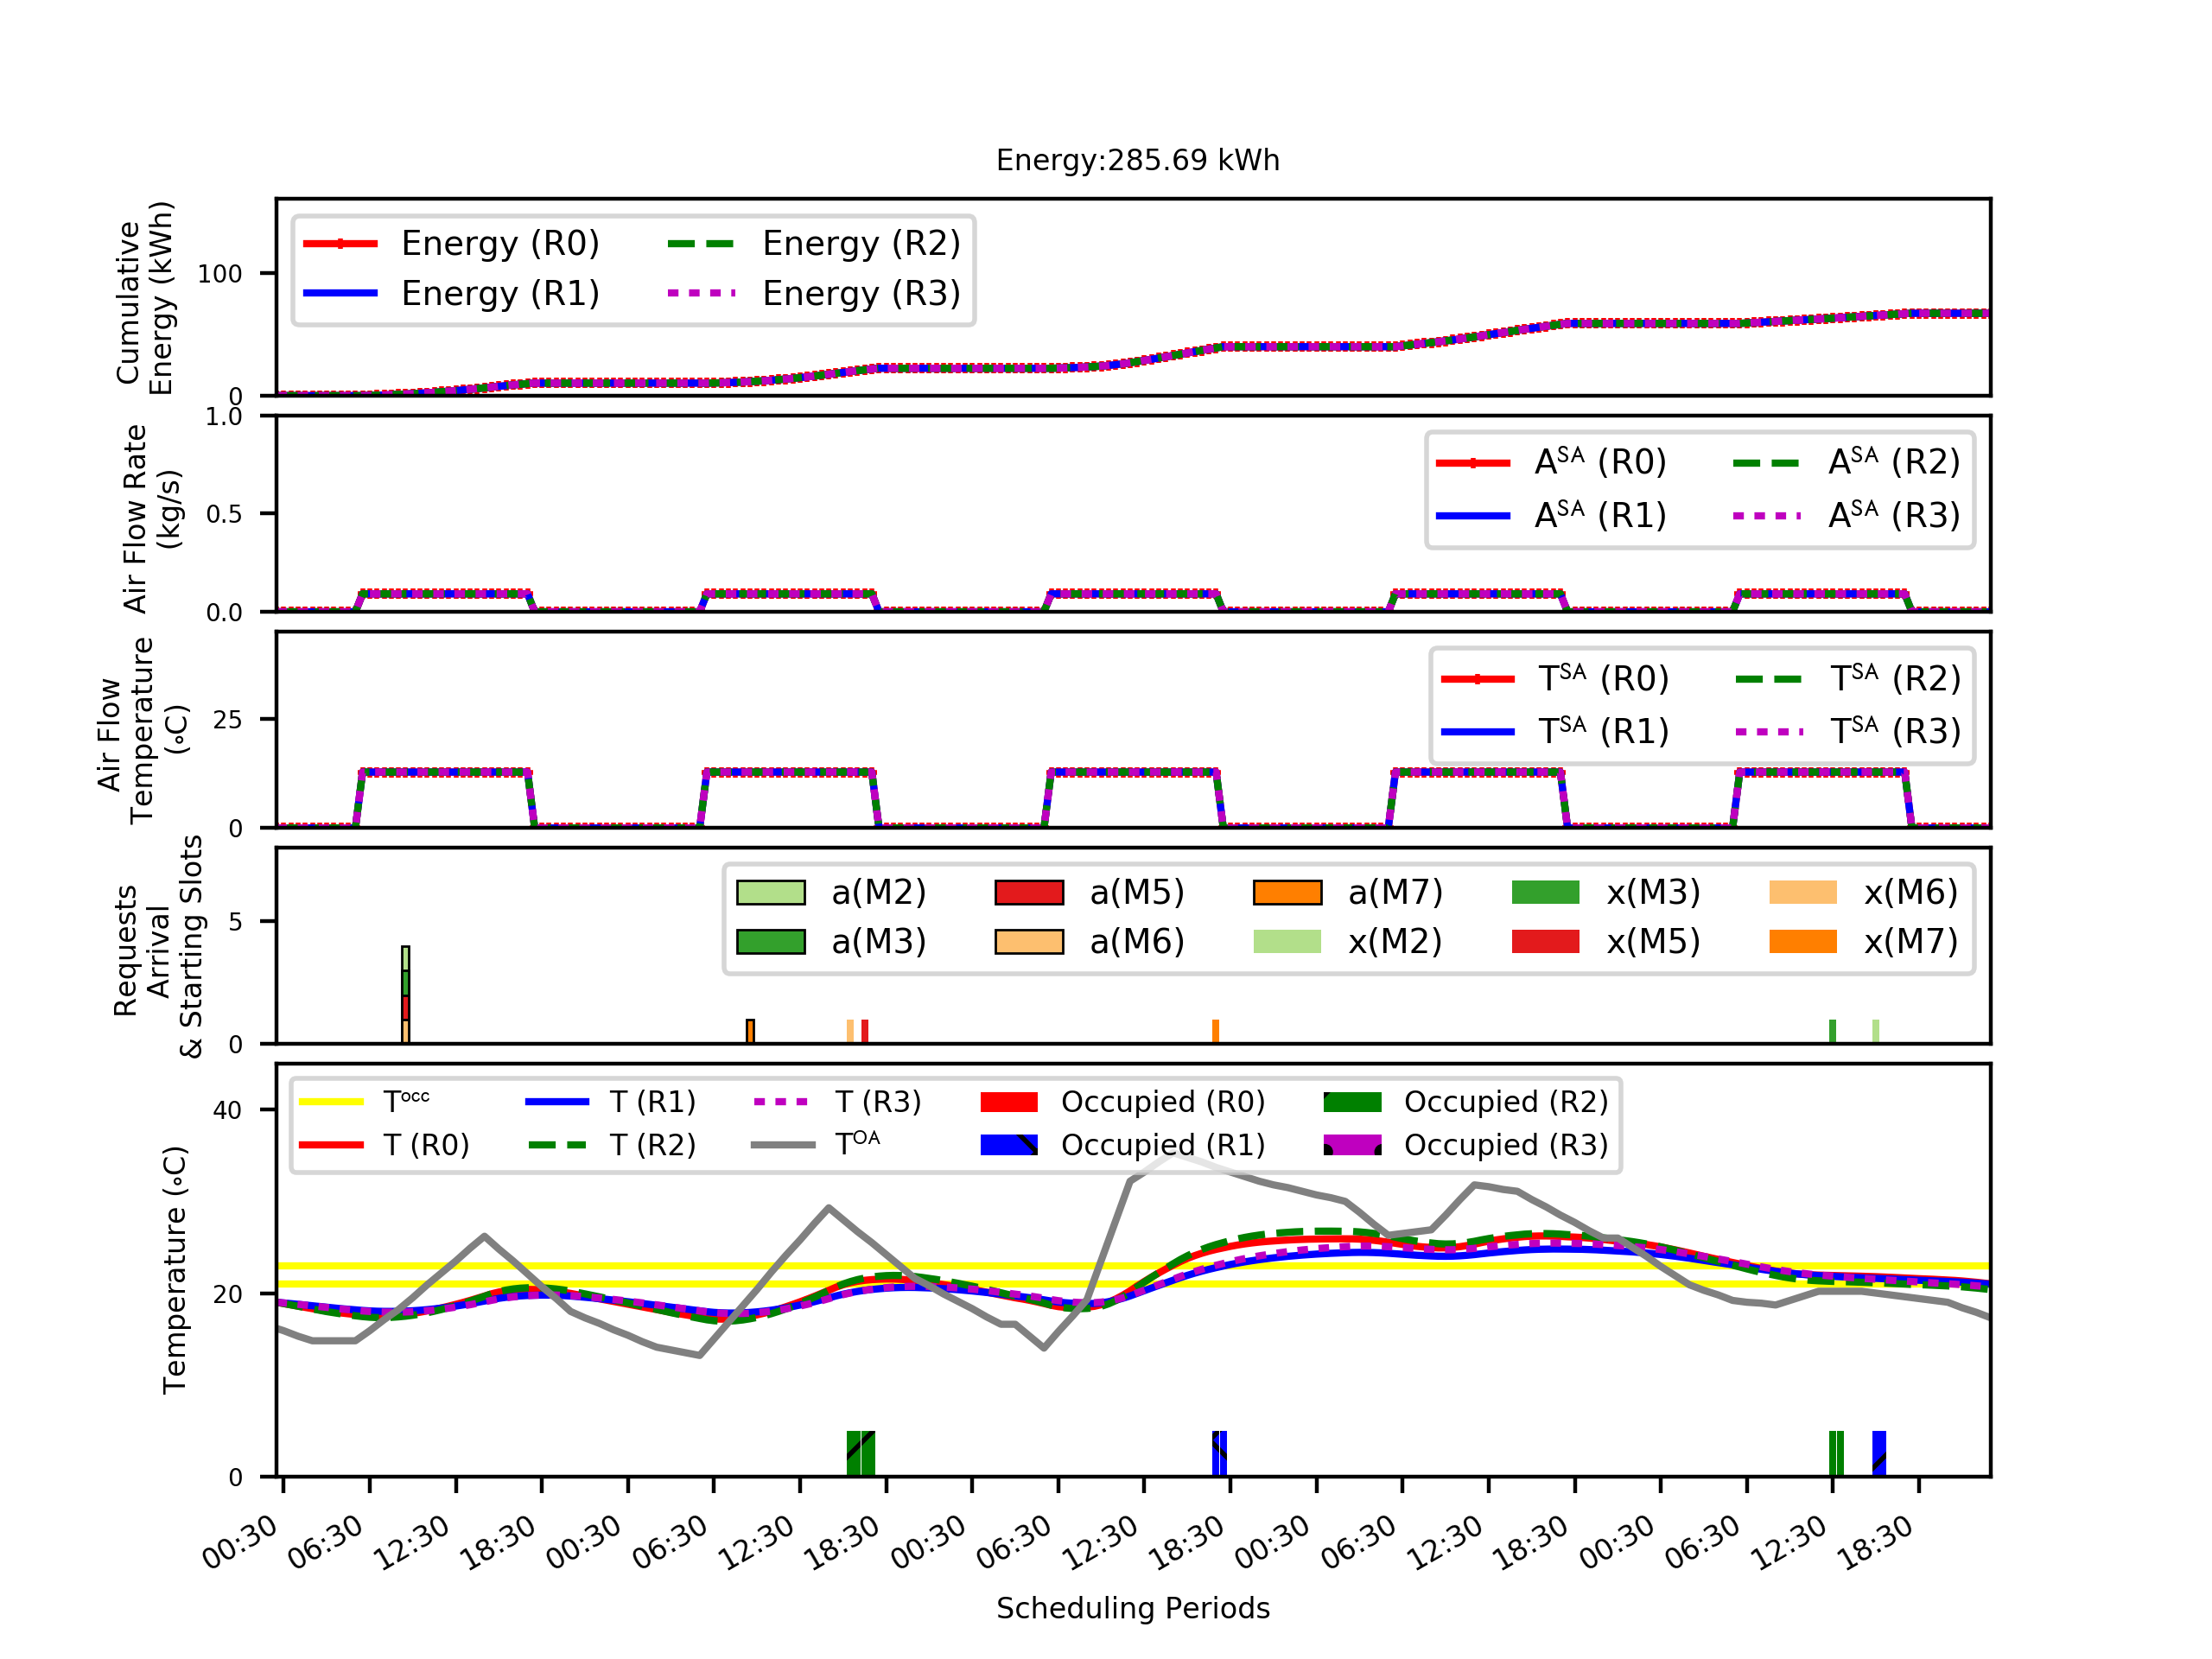
\includegraphics[width=0.9\linewidth]{figs/online_r1.png}
    %\caption{Online Scheduling - Session 2}
    %\label{fig:online_eg2}
%\end{sidewaysfigure}
%
%\begin{sidewaysfigure}[h]
    %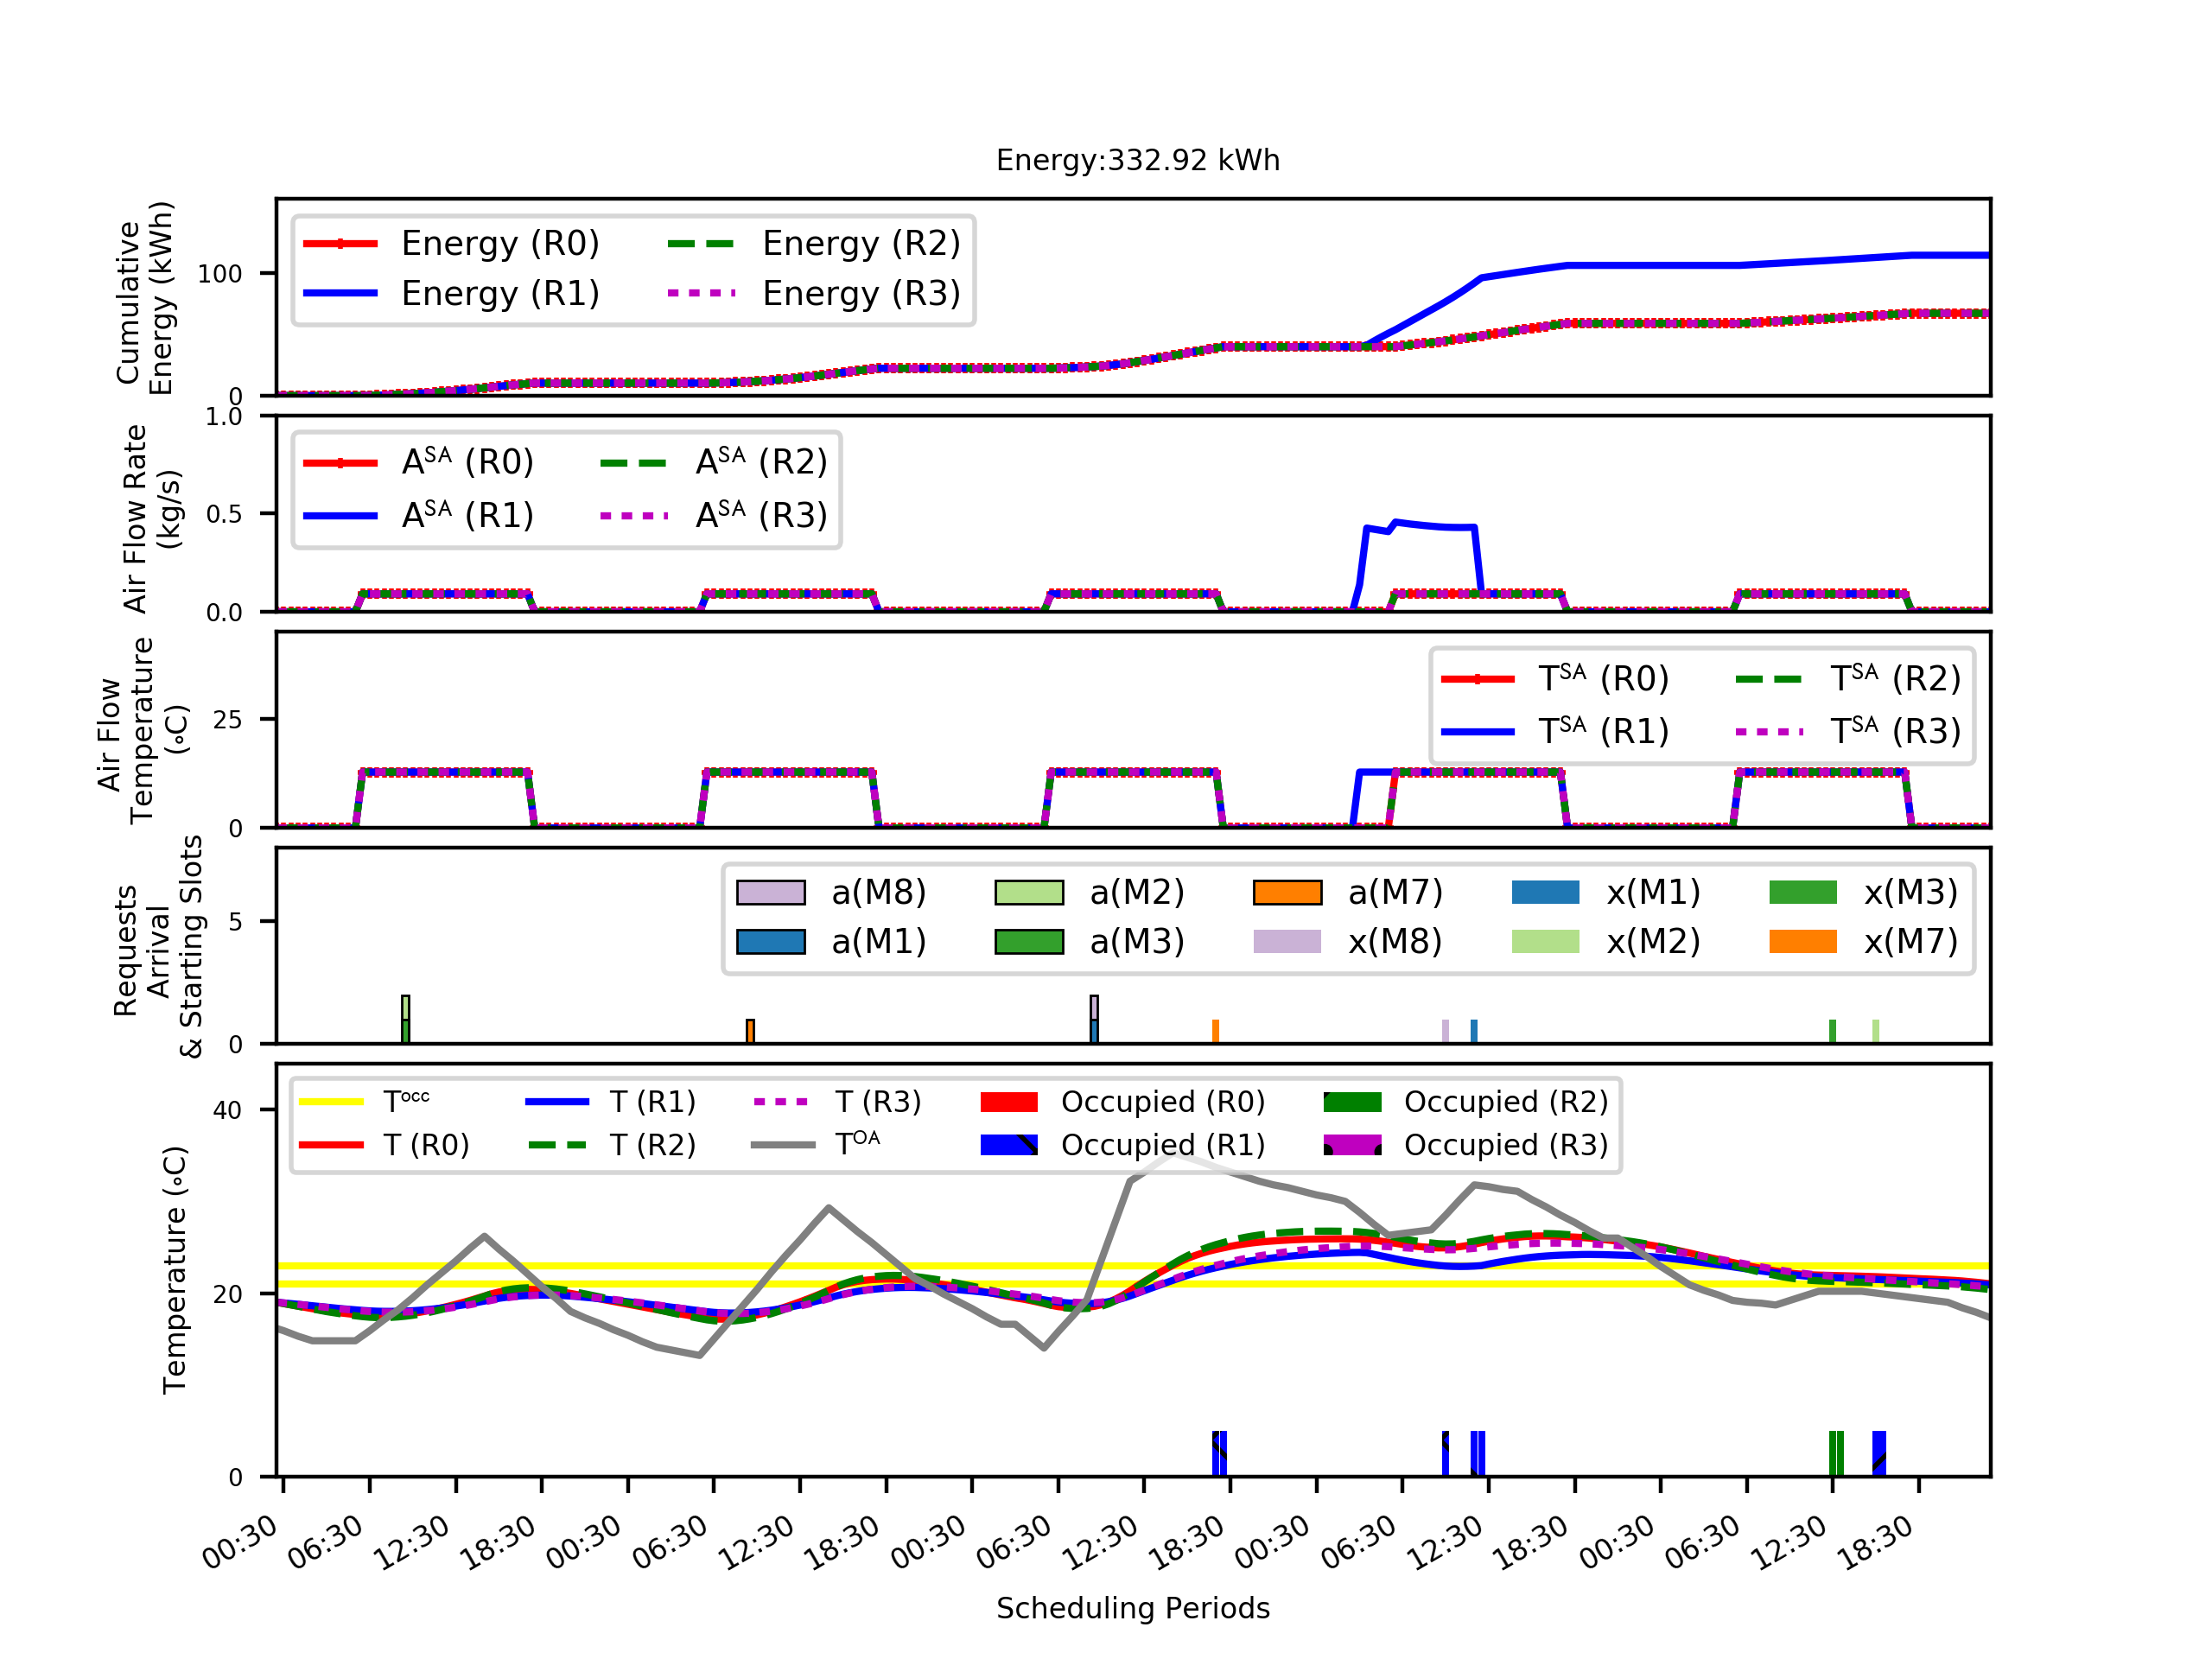
\includegraphics[width=0.9\linewidth]{figs/online_r2.png}
    %\caption{Online Scheduling - Session 3}
    %\label{fig:online_eg3}
%\end{sidewaysfigure}
%
%\begin{sidewaysfigure}[h]
    %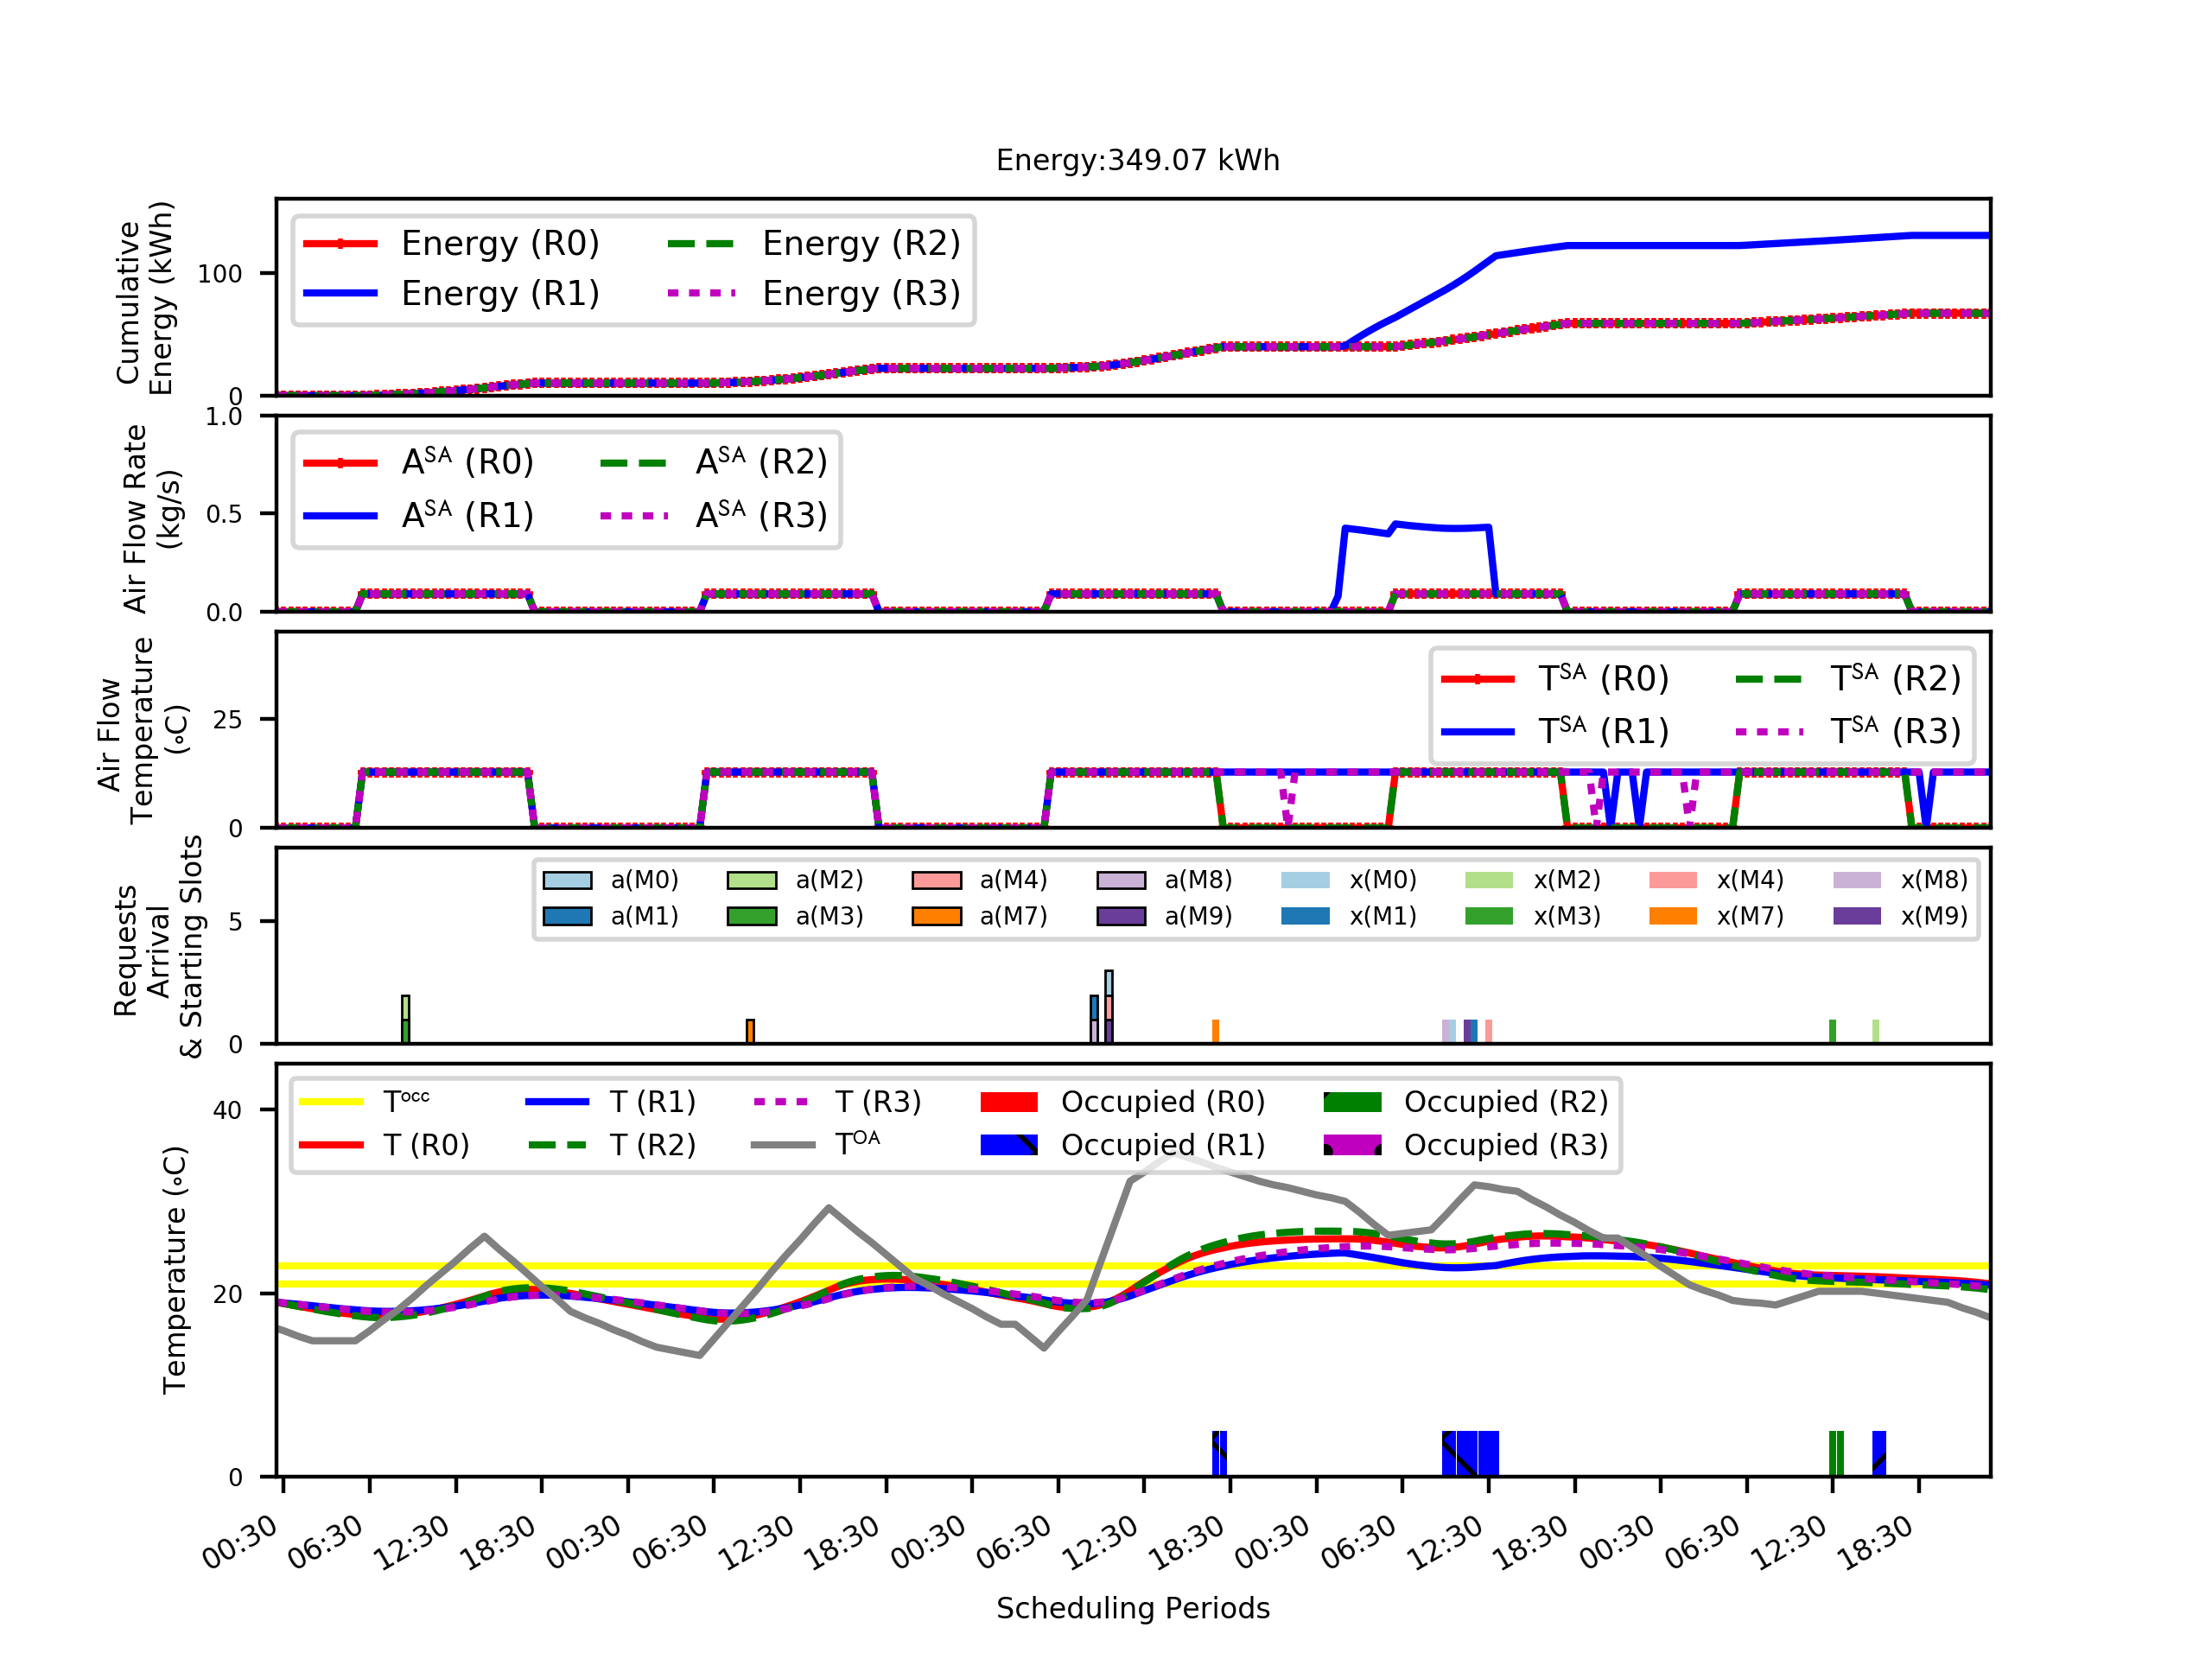
\includegraphics[width=0.9\linewidth]{figs/online_r3.png}
    %\caption{Online Scheduling - Session 4}
    %\label{fig:online_eg4}
%\end{sidewaysfigure}
%
%
%\begin{sidewaysfigure}[ht]
    %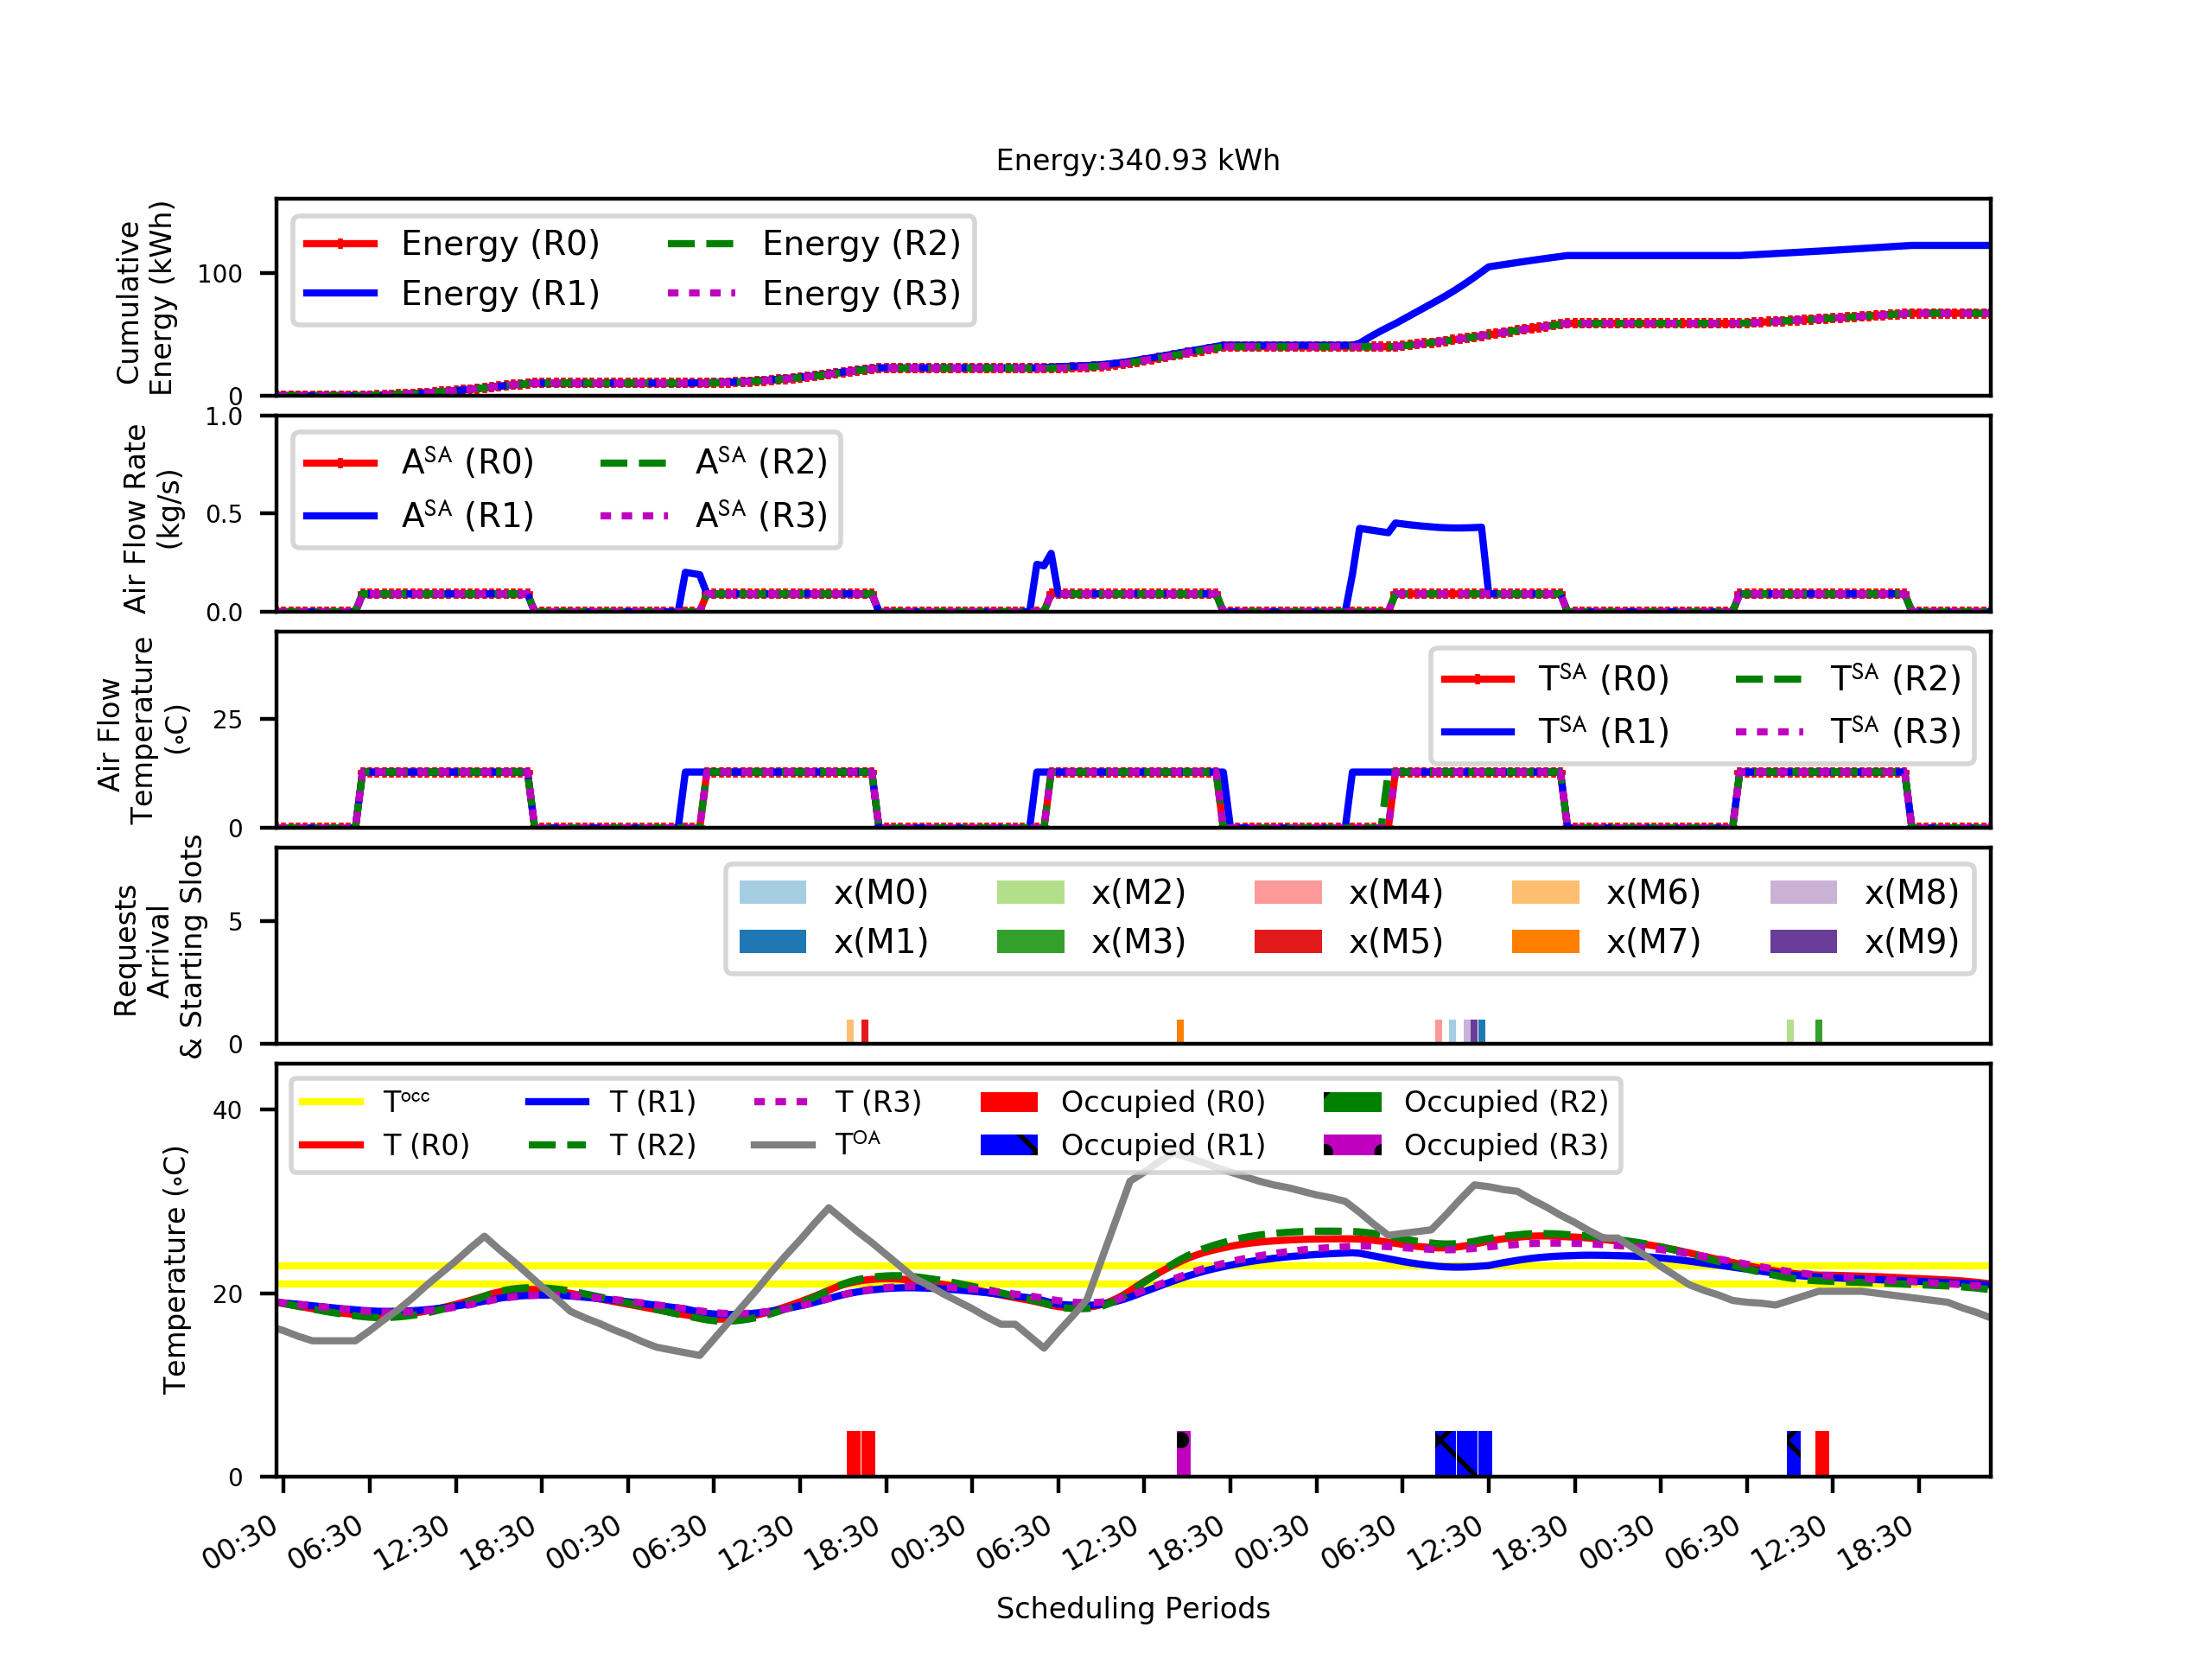
\includegraphics{figs/online_oracle.png}
    %\caption{Offline Scheduling}
    %\label{fig:online_offline}
%\end{sidewaysfigure}


\begin{figure}[t]
\centering
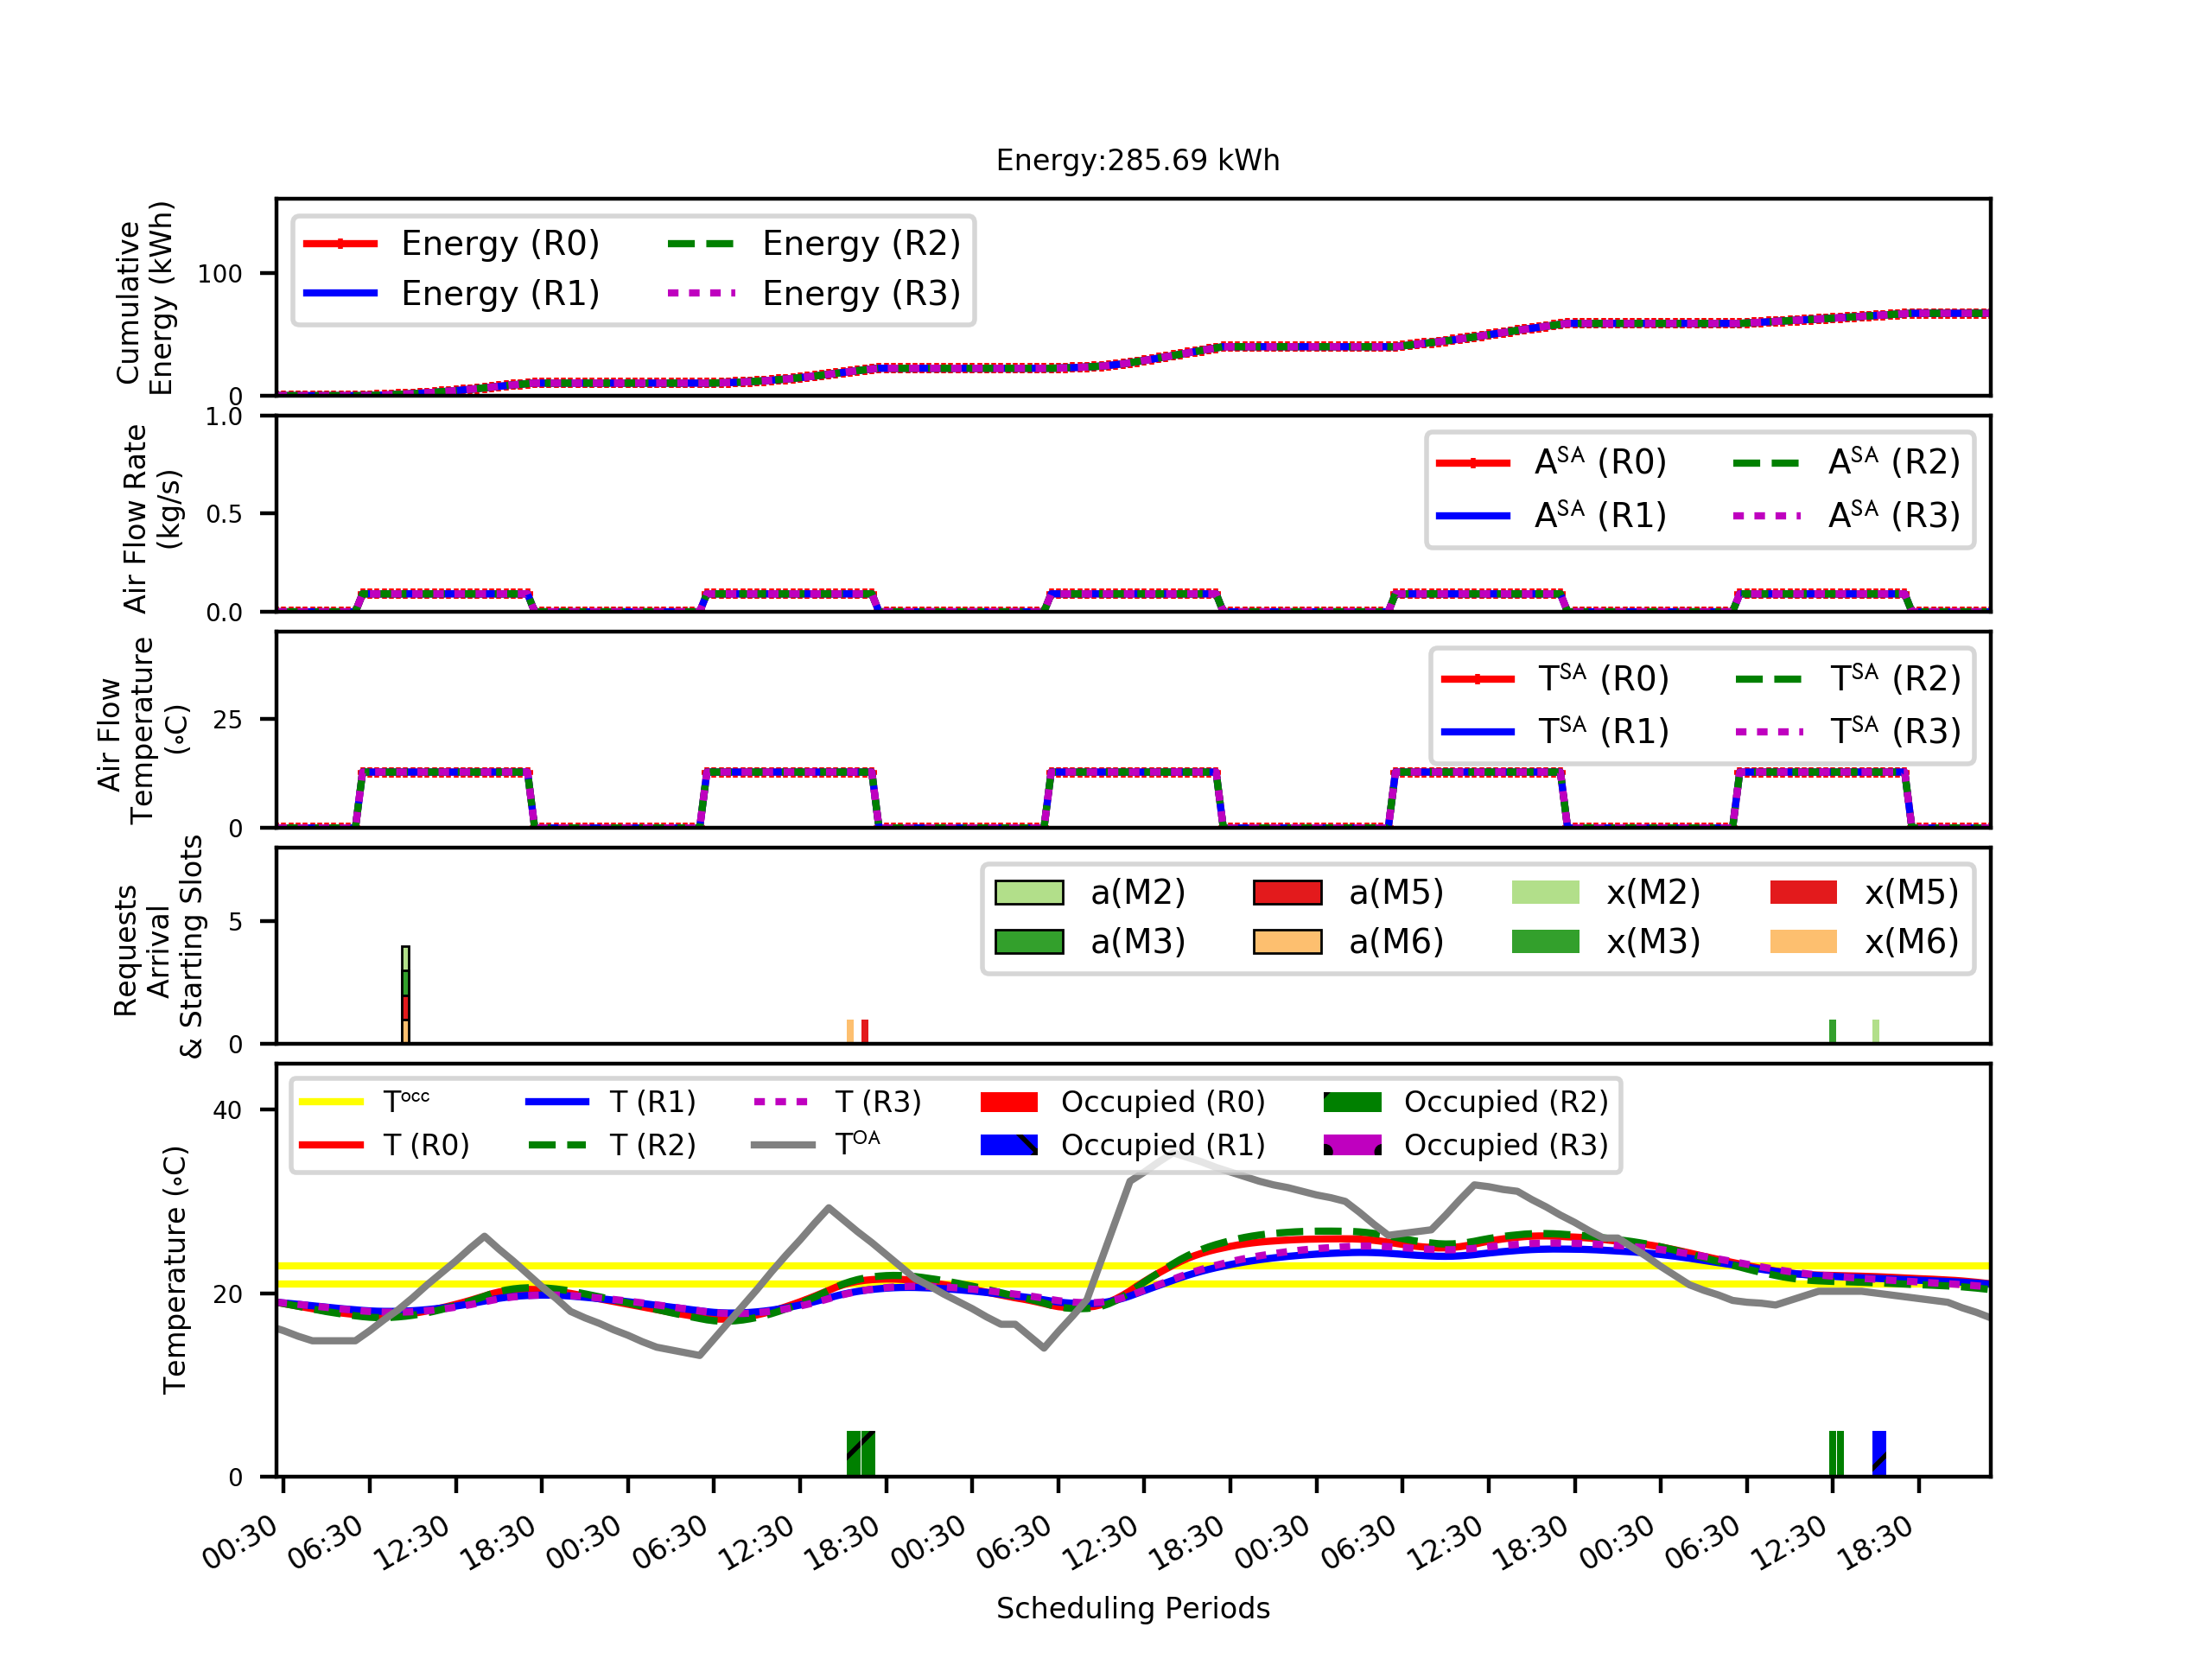
\includegraphics[width=1\linewidth]{figs/online_r0.png}	
\vspace*{-2ex}
\caption{Online scheduling scenario - Session 1}
\label{fig:online_eg1}
\end{figure}

\begin{figure}[t]
\centering
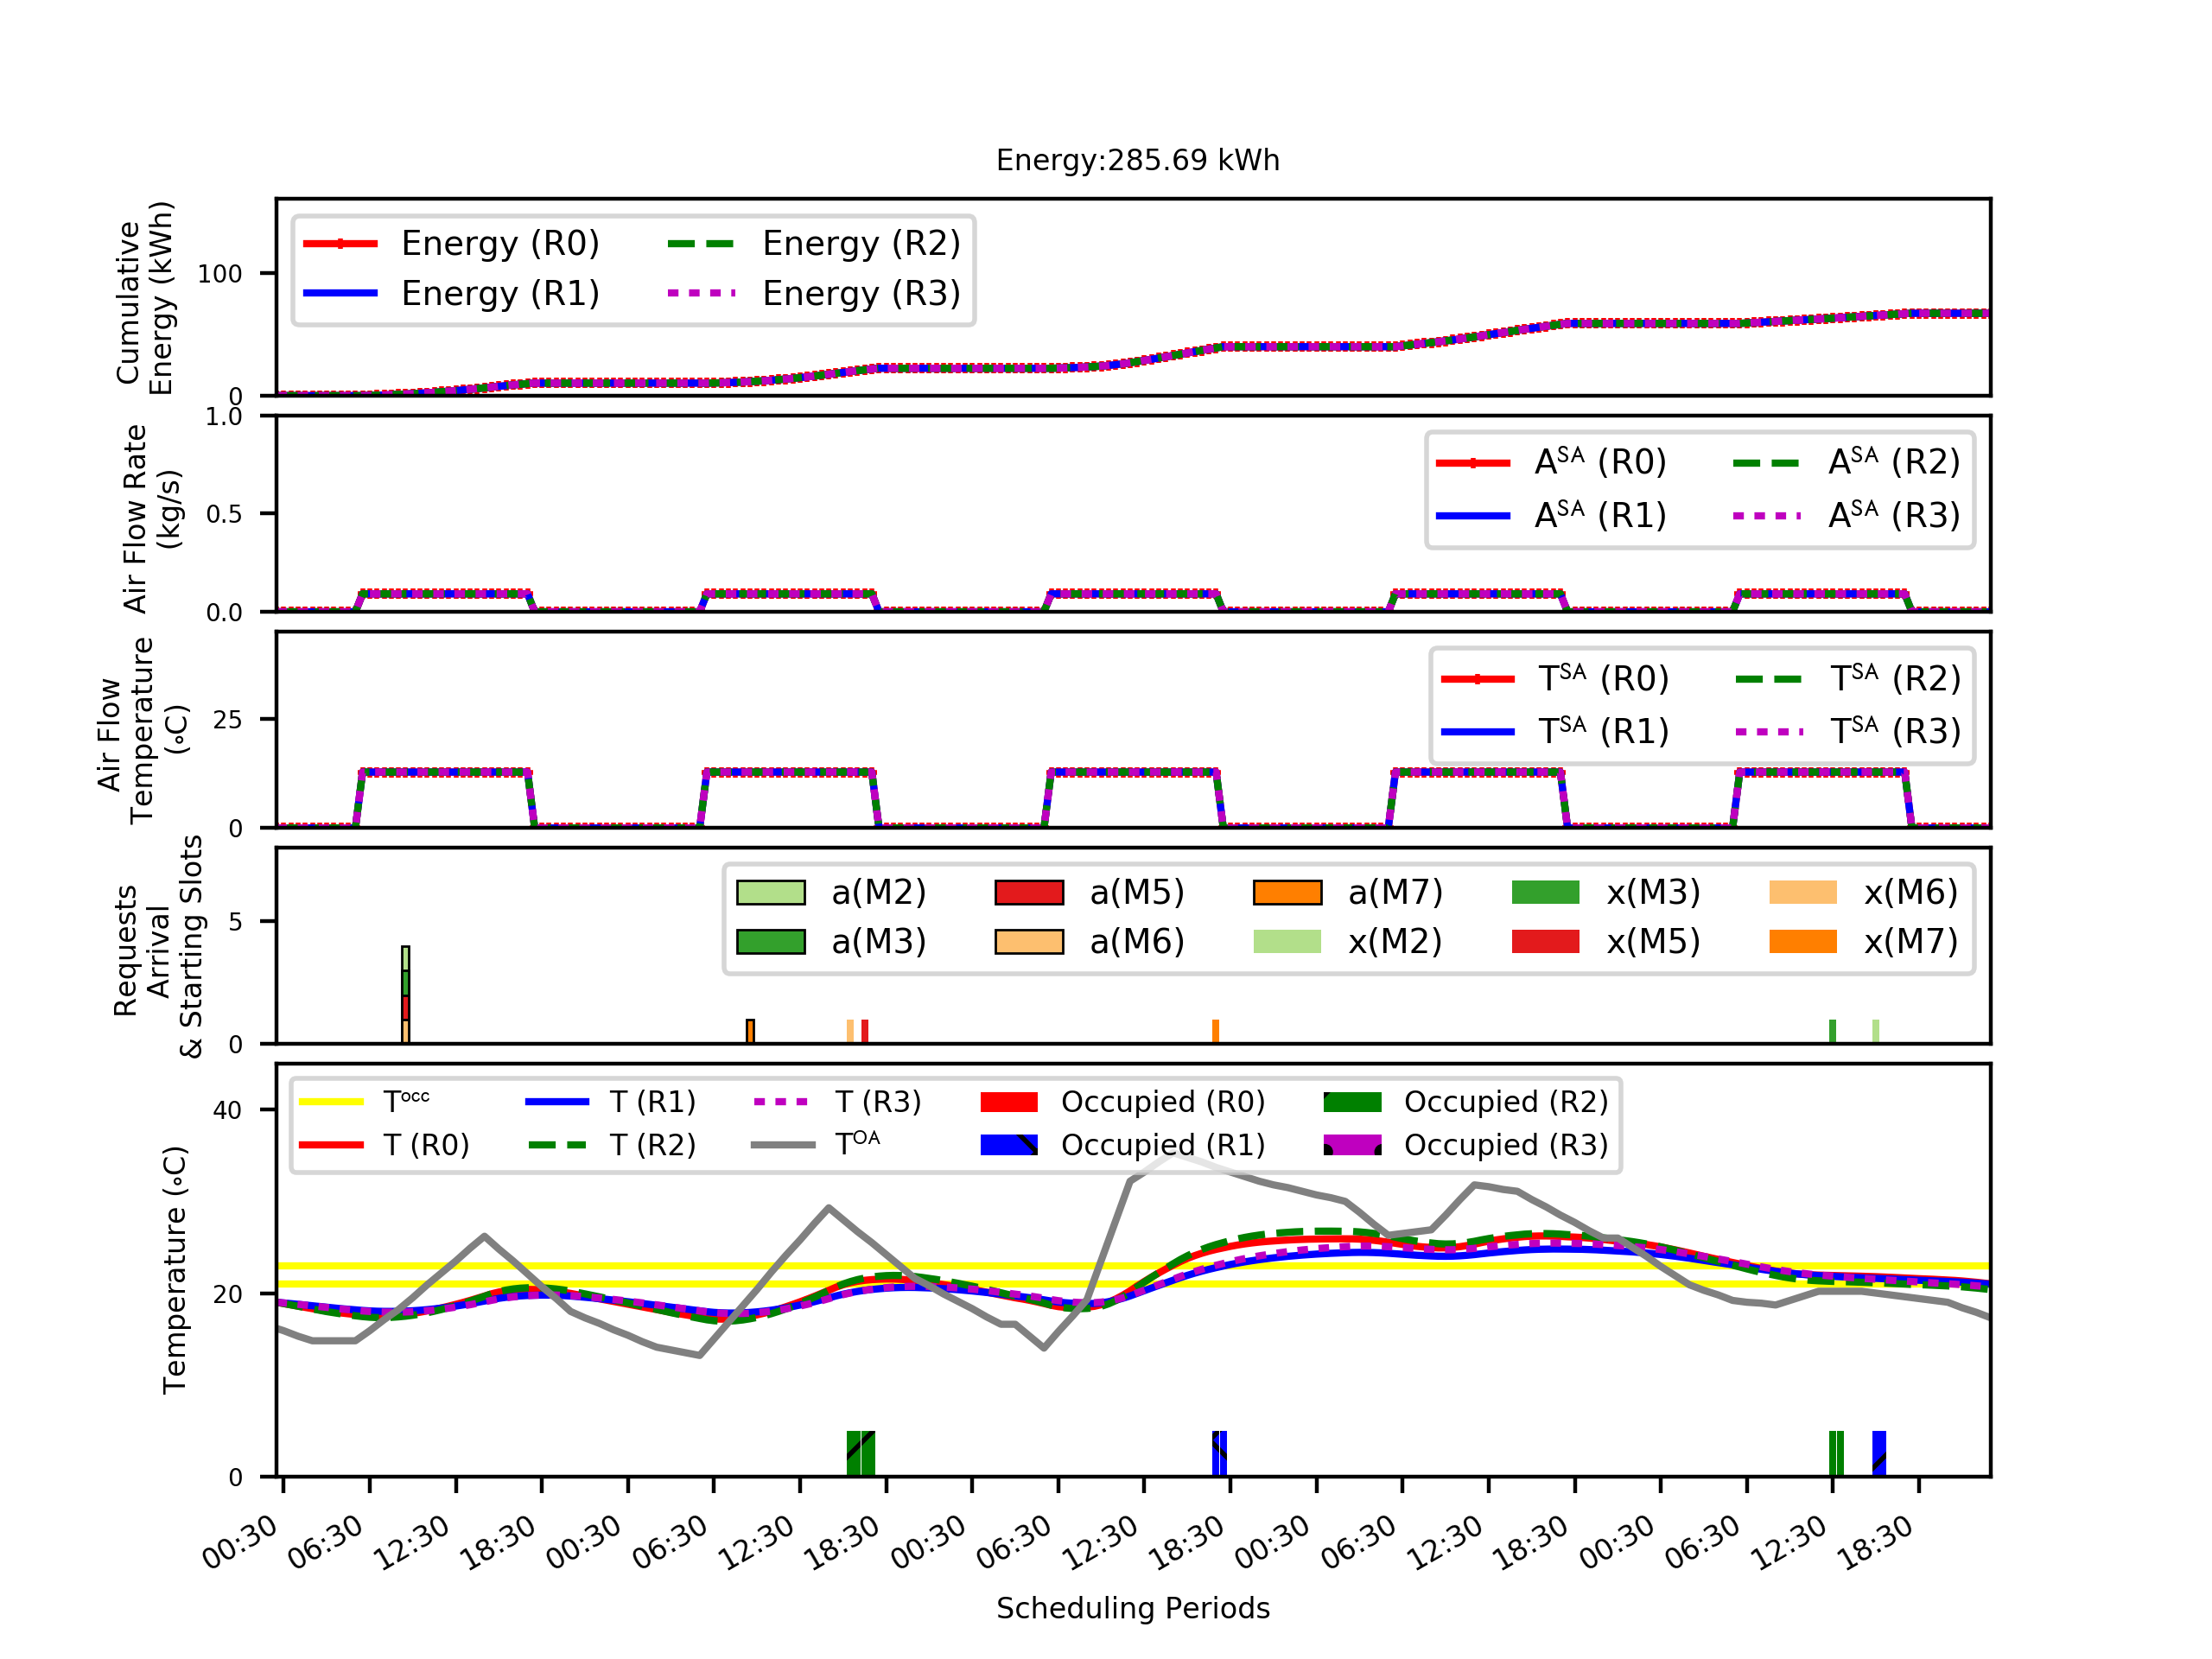
\includegraphics[width=1\linewidth]{figs/online_r1.png}	
\vspace*{-2ex}
\caption{Online scheduling scenario - Session 2}
\label{fig:online_eg2}
\end{figure}


\begin{figure}[t]
\centering
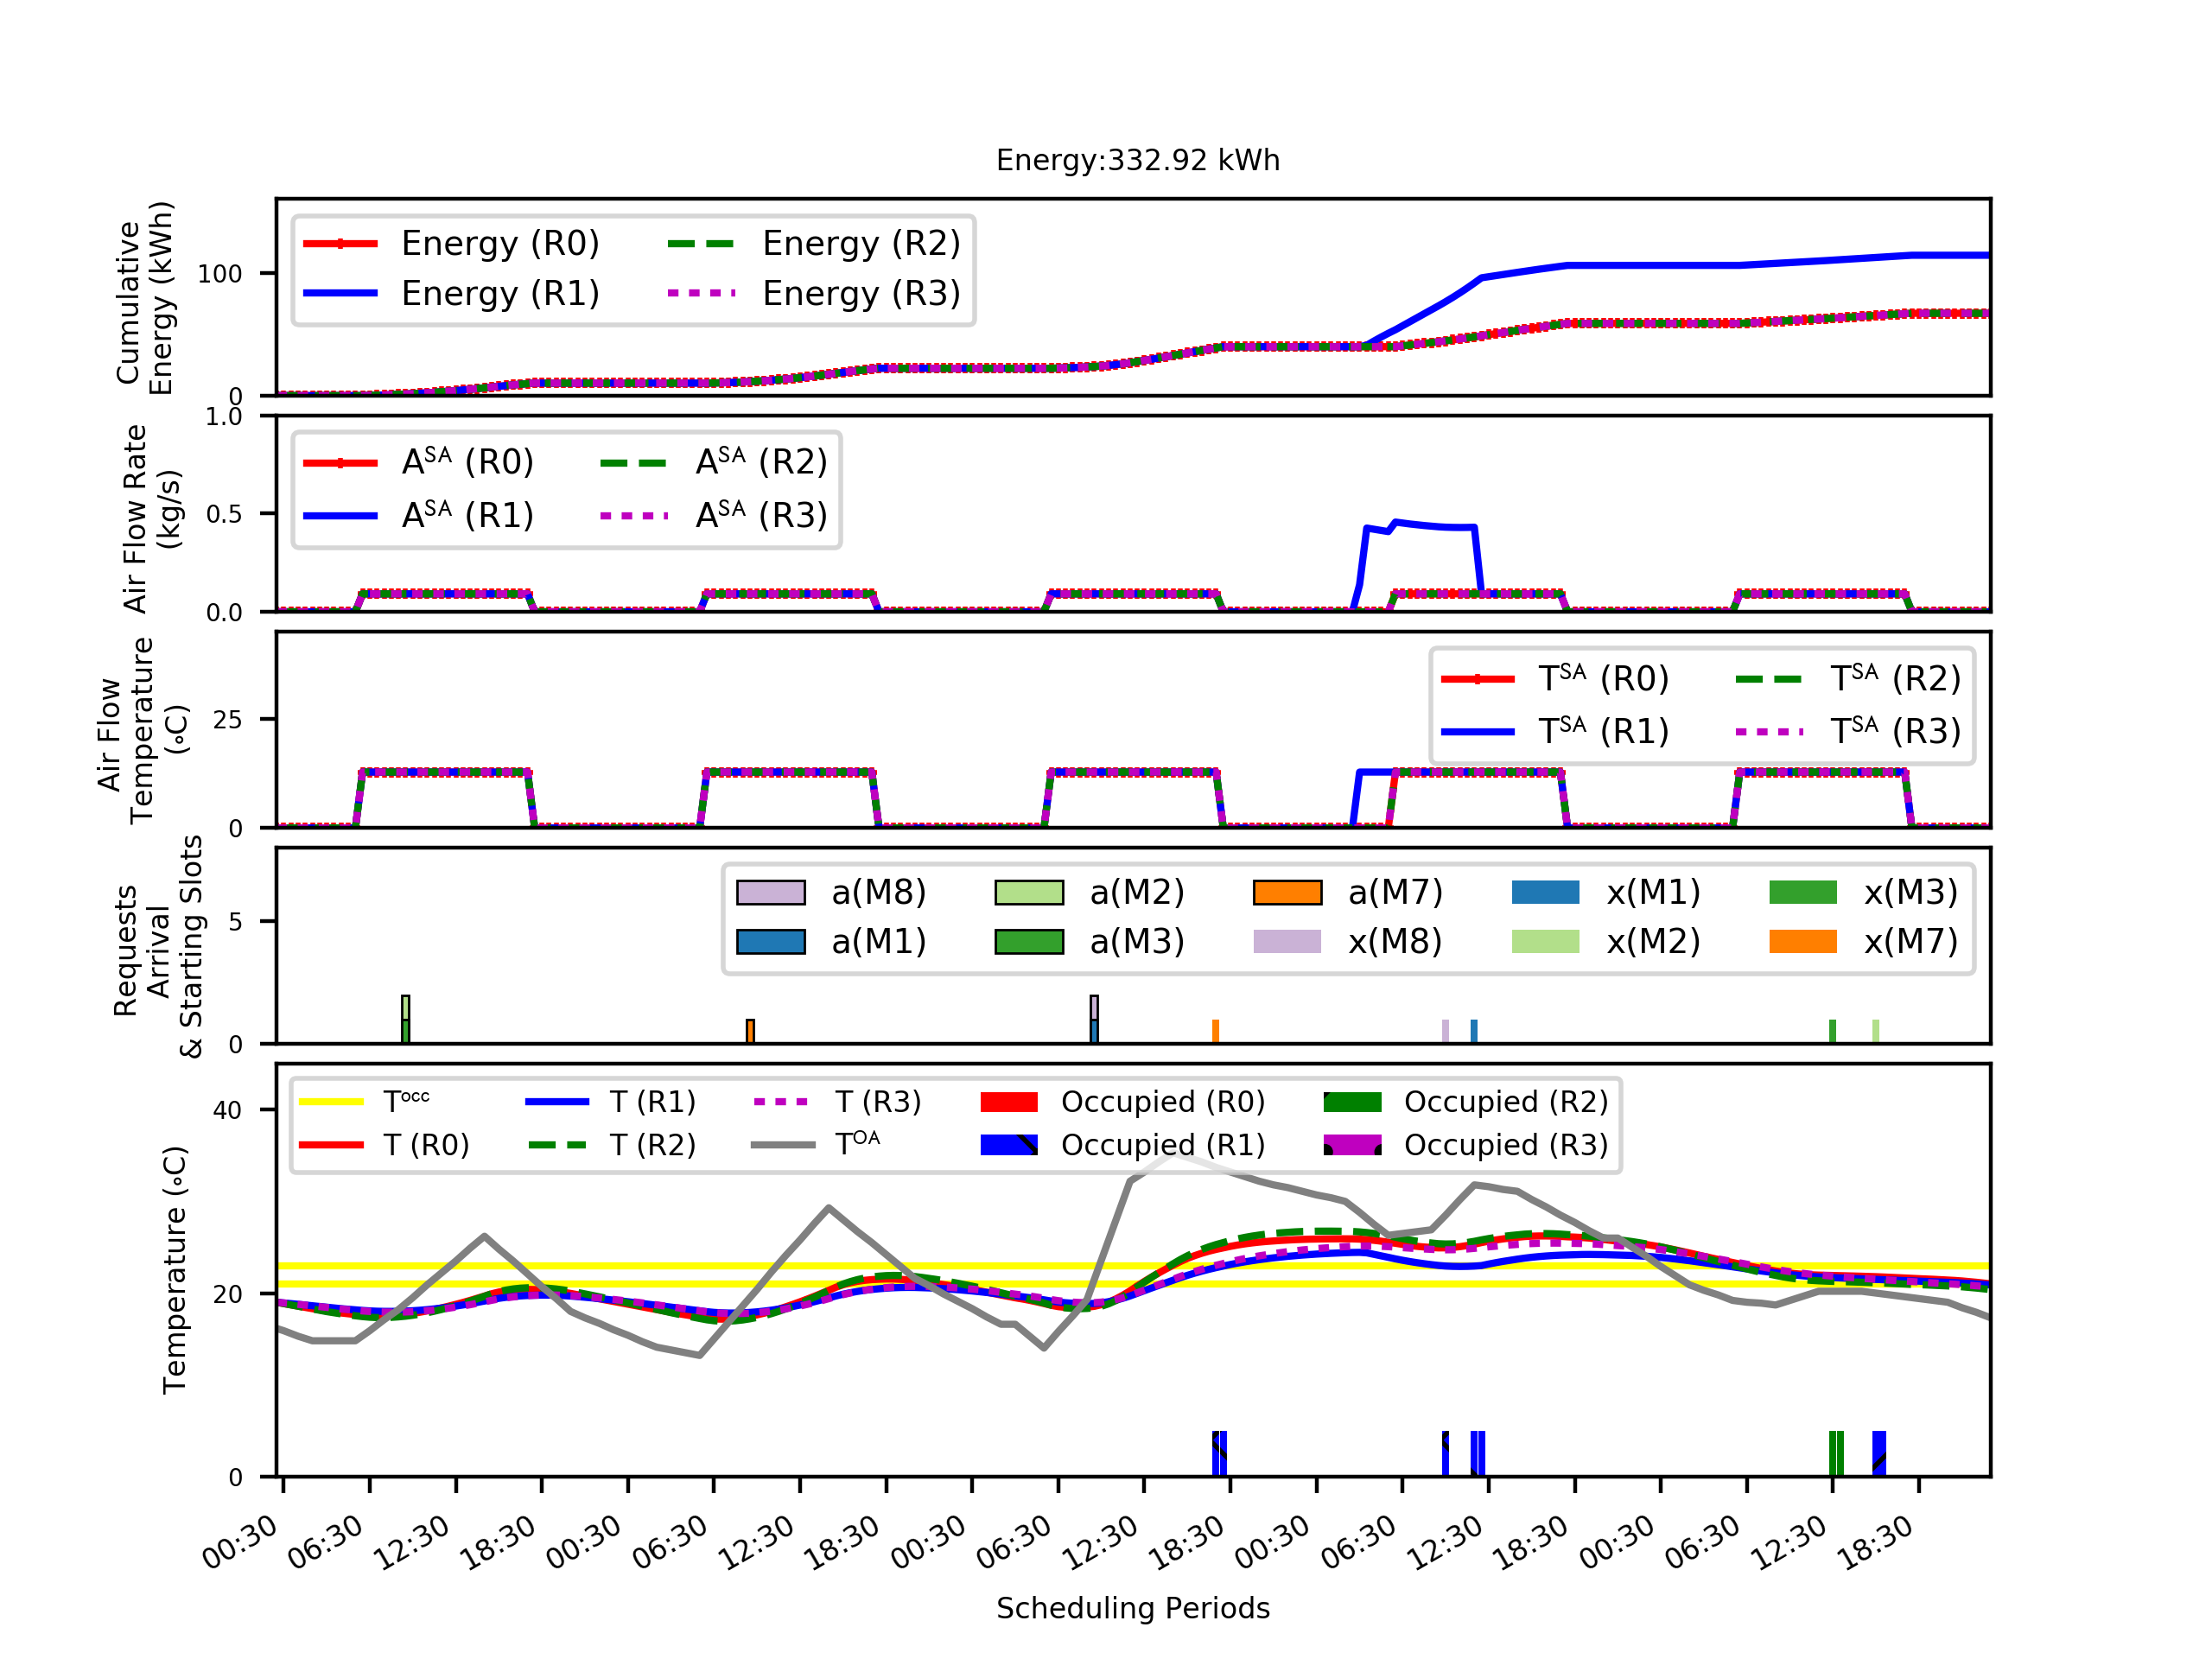
\includegraphics[width=1\linewidth]{figs/online_r2.png}	
\vspace*{-2ex}
\caption{Online scheduling scenario - Session 3}
\label{fig:online_eg3}
\end{figure}

\begin{figure}[t]
\centering
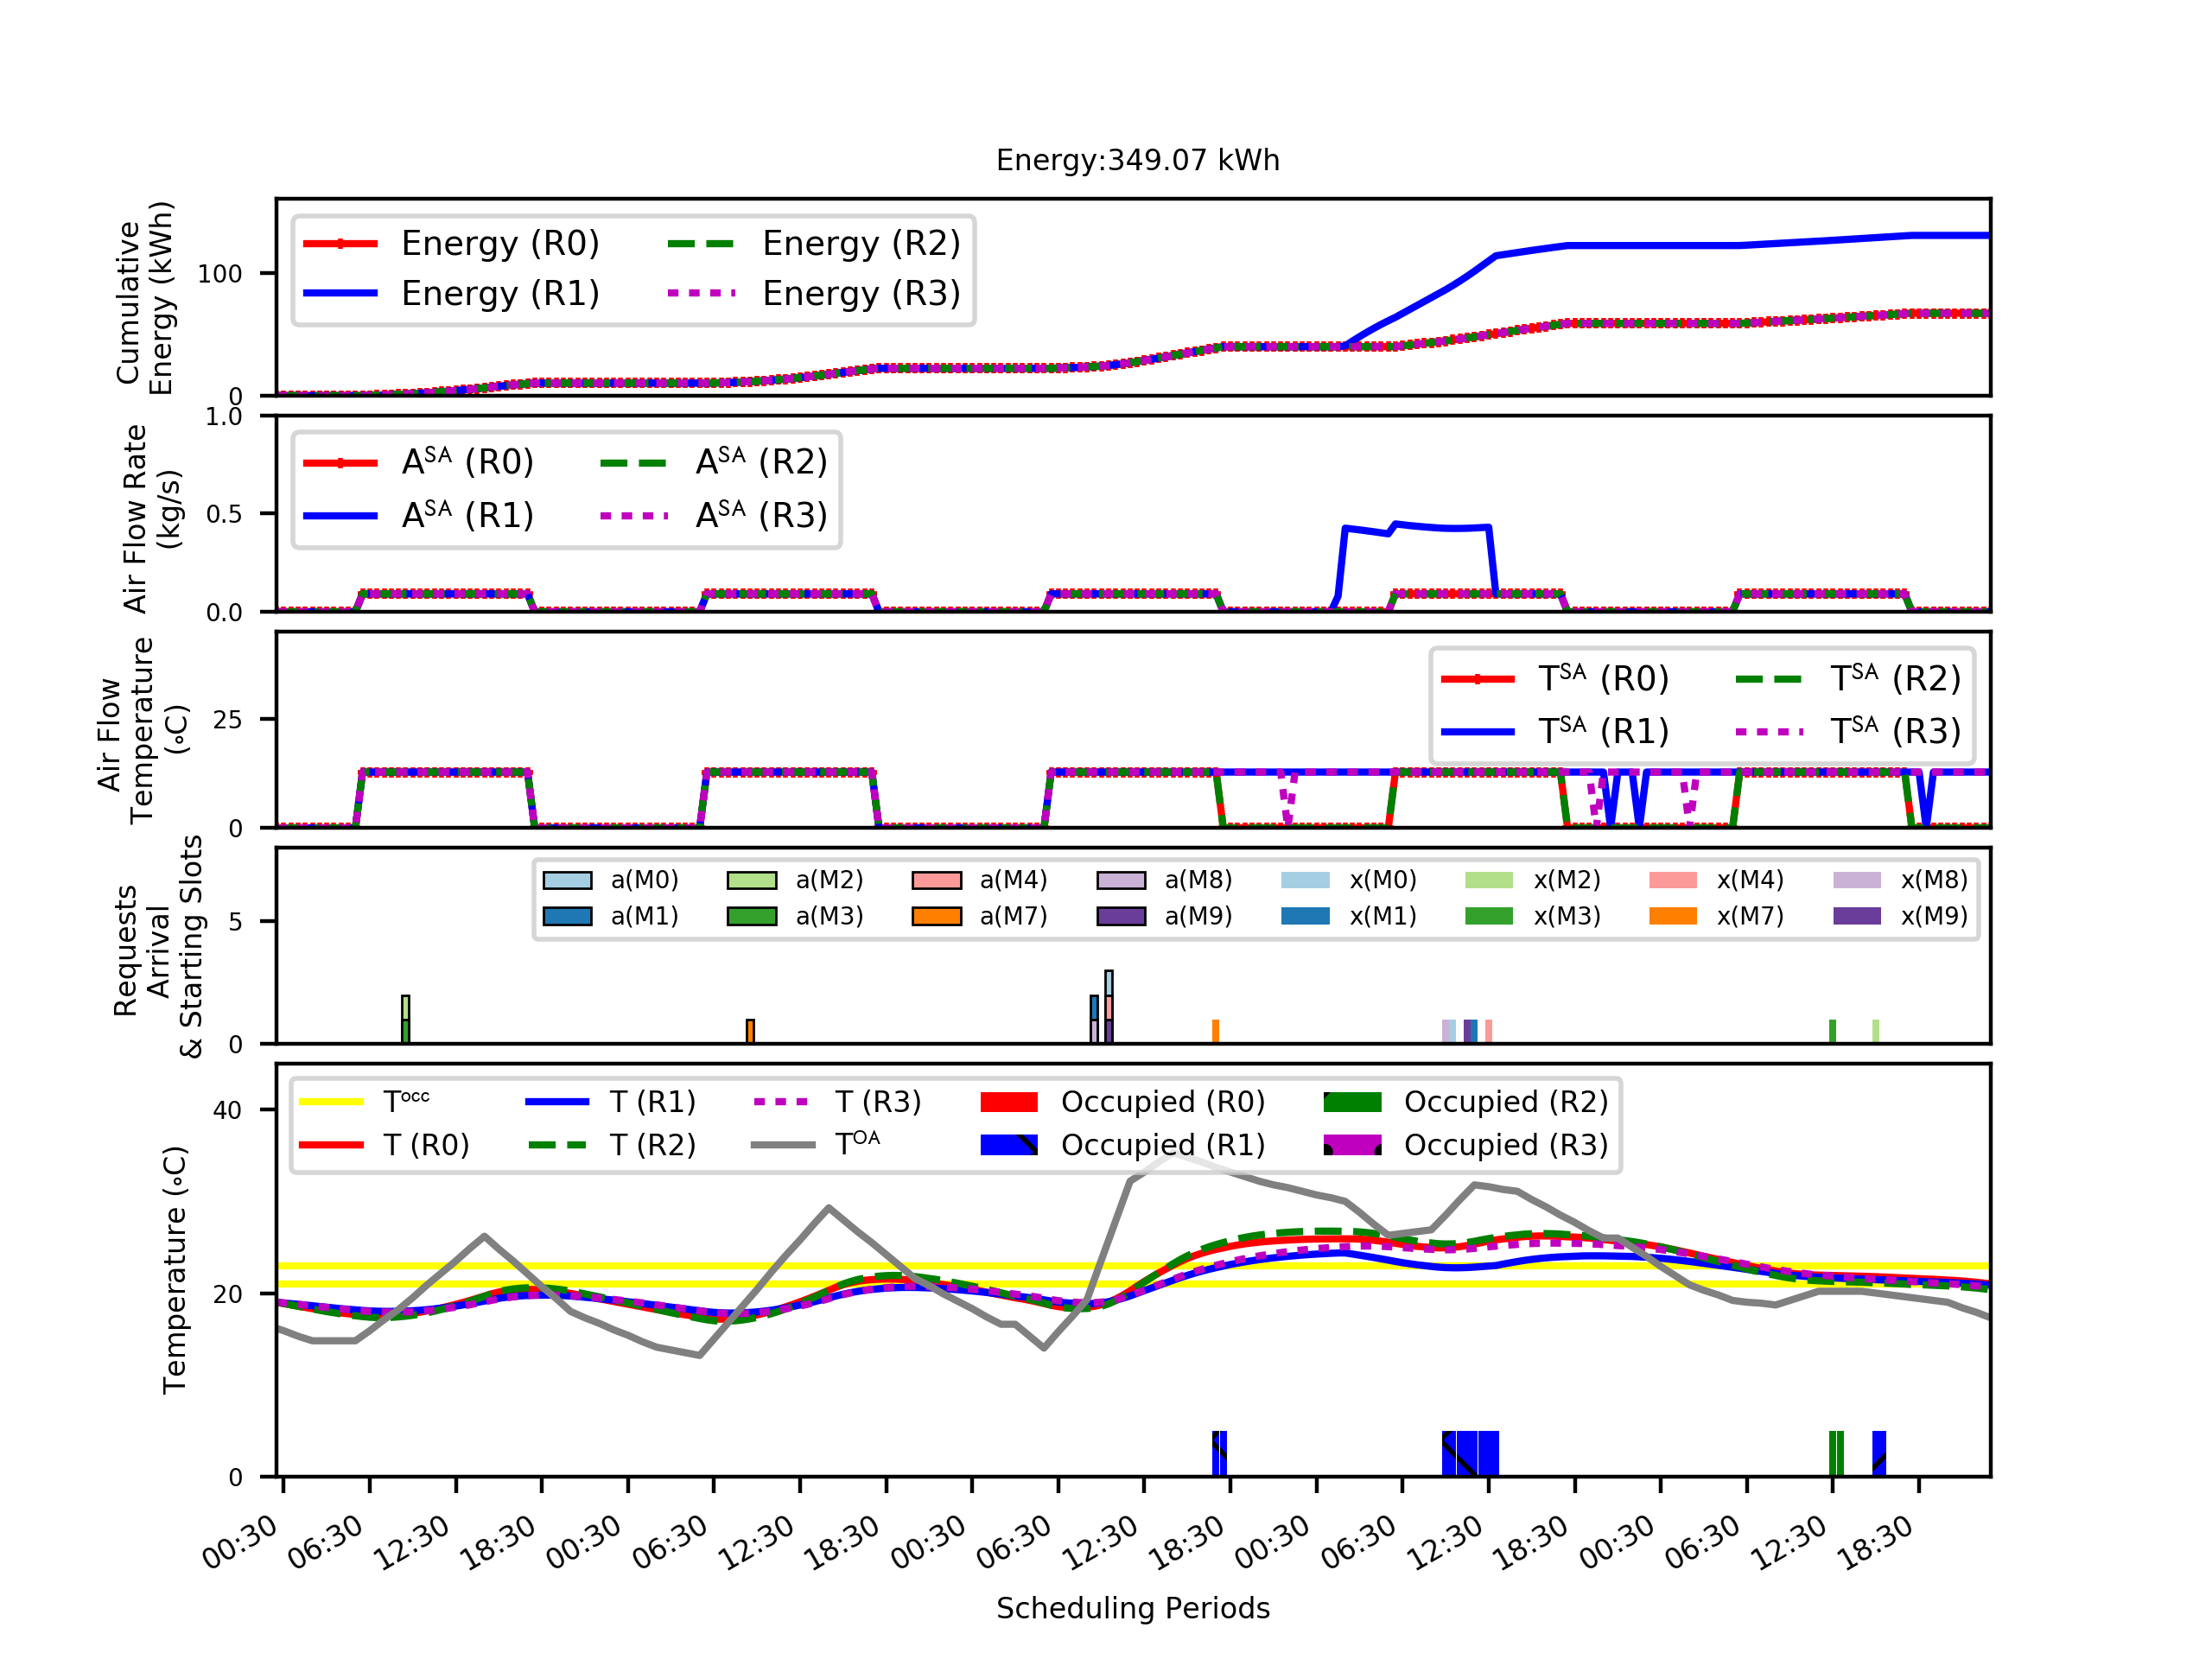
\includegraphics[width=1\linewidth]{figs/online_r3.png}	
\vspace*{-2ex}
\caption{Online scheduling scenario - Session 4}
\label{fig:online_eg4}
\end{figure}

\begin{figure}[t]
\centering
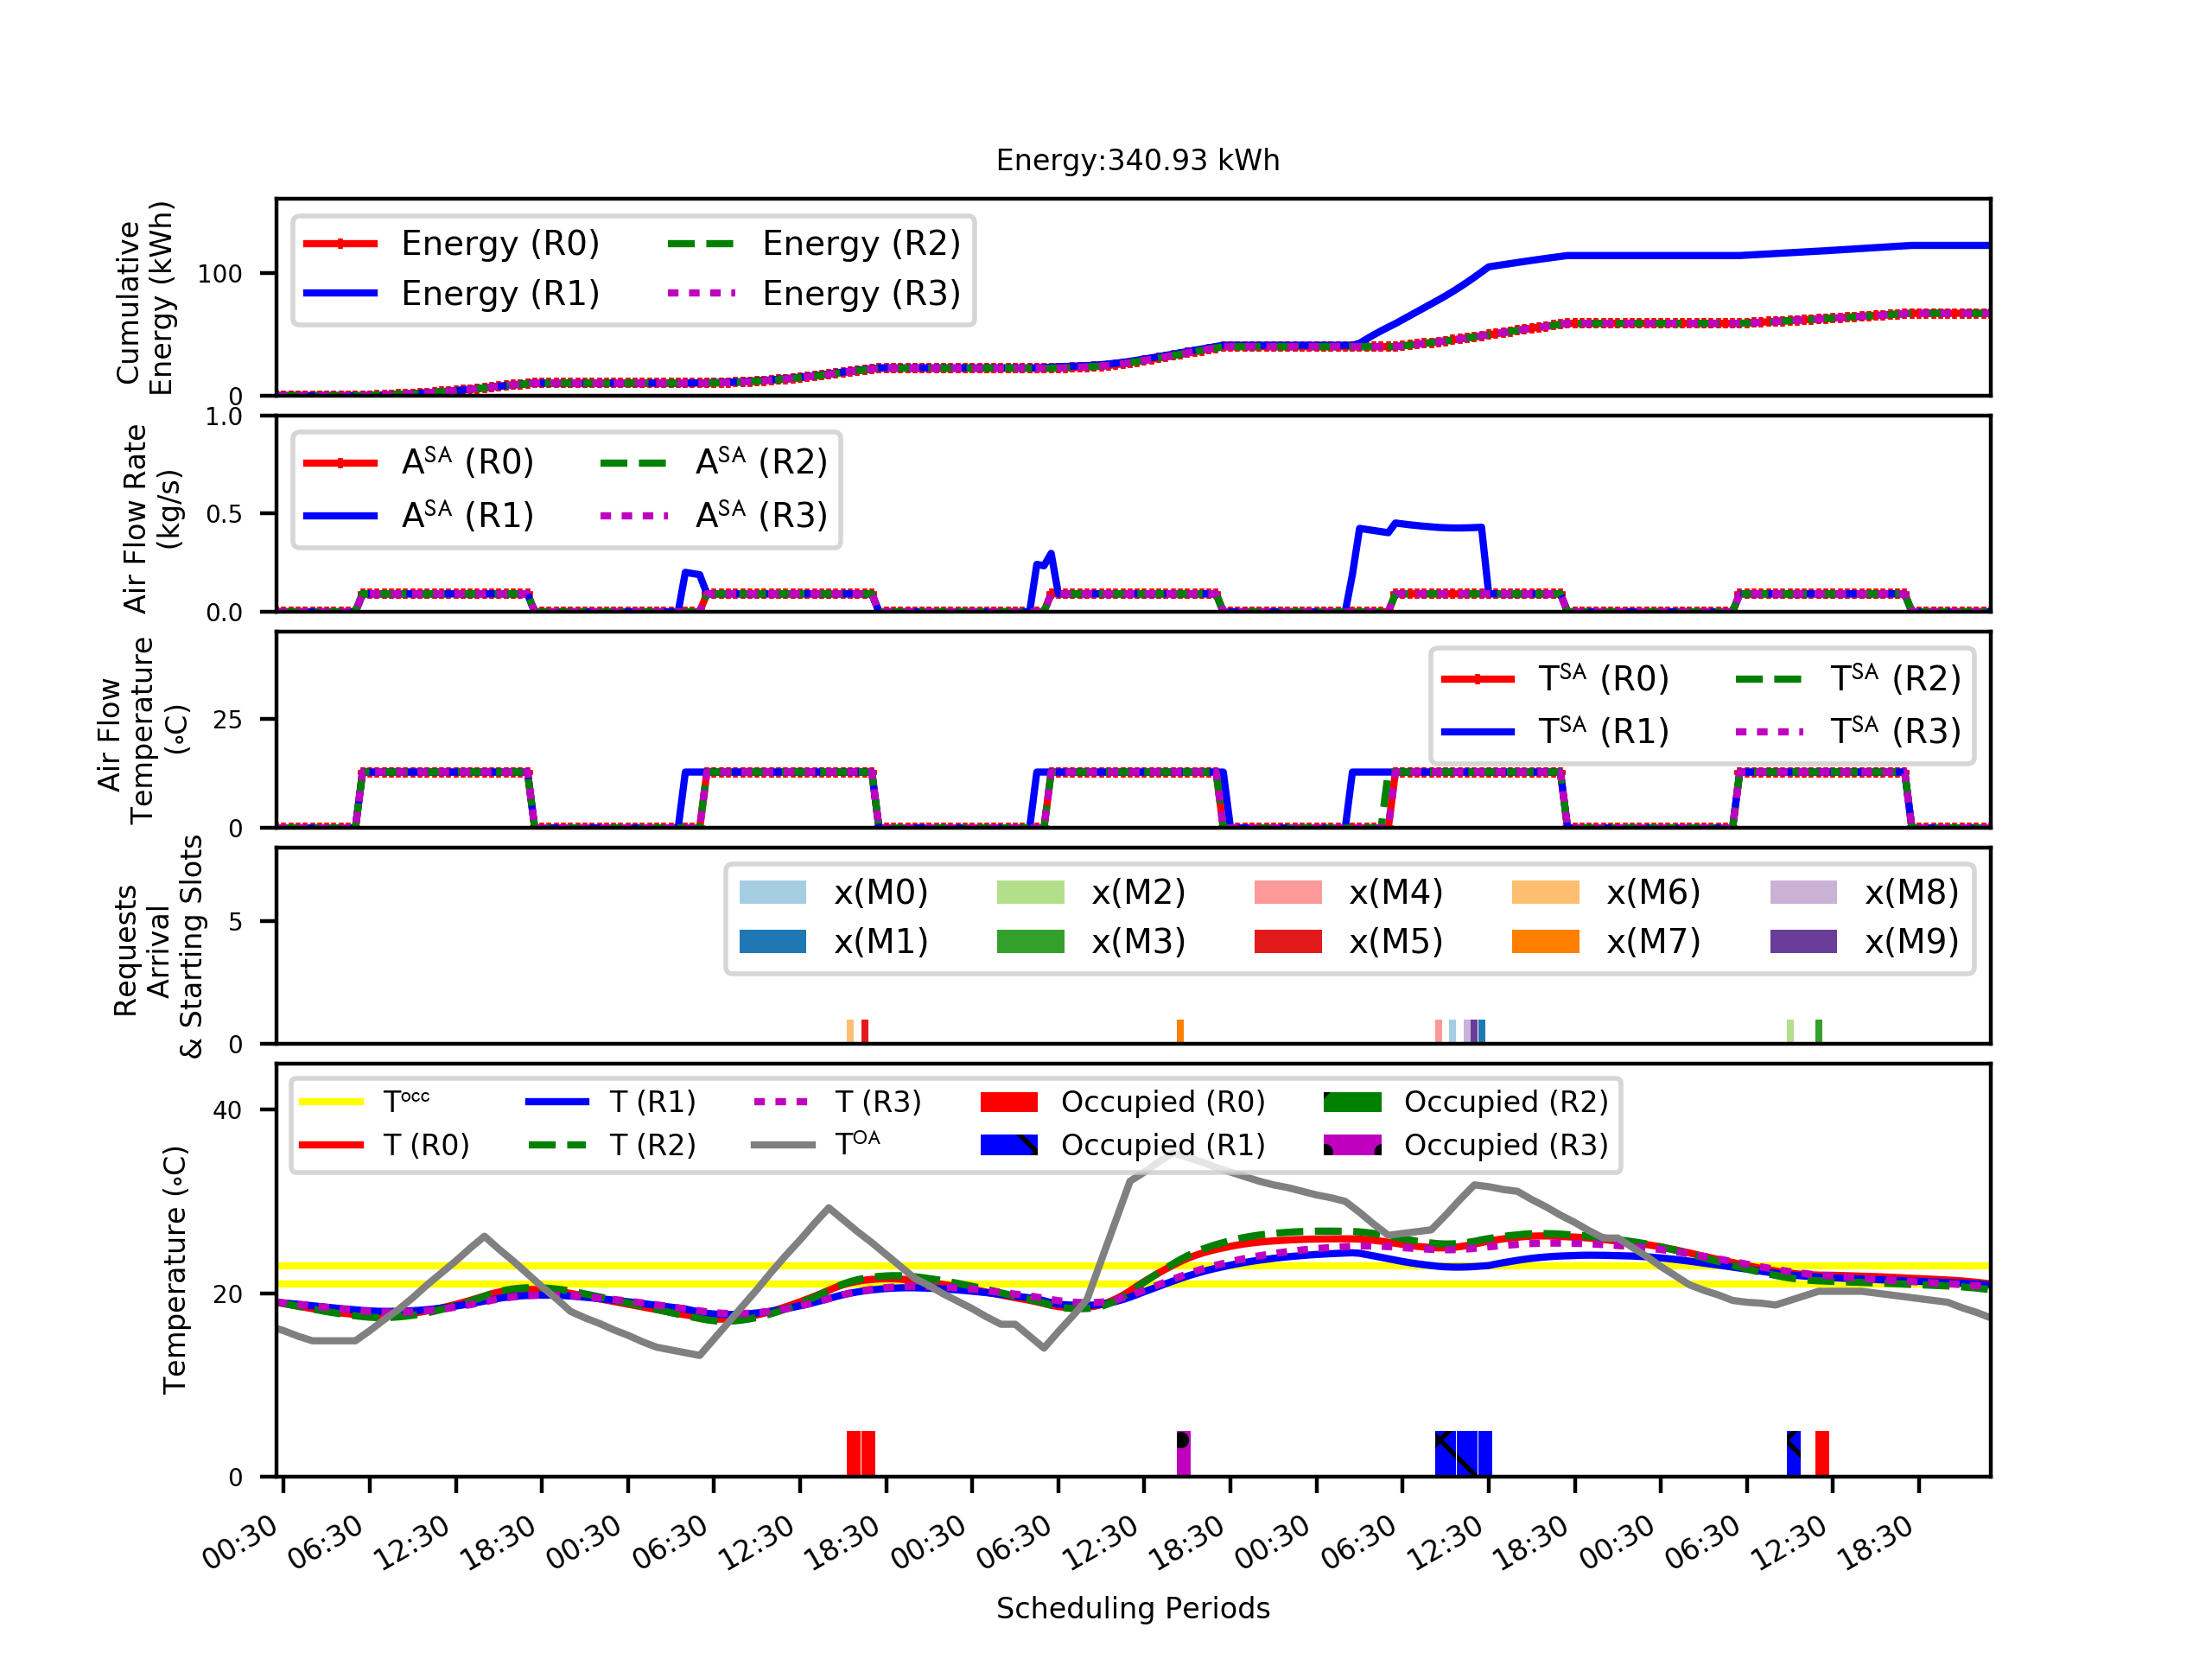
\includegraphics[width=1\linewidth]{figs/online_oracle.png}	
\vspace*{-2ex}
\caption{Offline scheduling scenario}
\label{fig:online_offline}
\end{figure}

Figures \ref{fig:online_eg1}-\ref{fig:online_eg4} show a scenario example of our online HVAC-aware occupancy scheduling. In each figure, from the top, the first sub-graph shows the cumulative energy consumption for each location over the scheduling horizon, the second and third sub-graphs depict the supply air flow rate and air flow temperature for each location, 
%the fourth sub-graph shows the time slots where requests arrive (bar with back stripe) and the time slots where the corresponding meetings start. The arrival time slot and the start time slot for the same meeting are assigned the same color.
the fourth sub-graph illustrates the time slots where requests arrive (bar with black border) and that of meetings start (bar with transparent border). The arrival time slot and the start time slot for the same meeting are assigned with the same color. 
Finally, the fifth sub-graph presents the rooms' temperatures and their occupied status.
For illustration purposes, we plot only the new meeting requests, as well as all ongoing and future activities that have been scheduled prior to the session. All meetings which had occurred prior to current session are removed. 

This scenario consists of 10 meetings $M \in \left\{M0, M1,\ldots, M9\right\}$, which are scheduled in 4 different online sessions. The set of locations is $L = \left\{R0, R1, R2, R3\right\}$. We set 5 minutes for the LNS runtime limit and 8.5 seconds for the MIP runtime during each repair step. For simplicity, we present the graphs in a finite horizon consisting of 240 steps, and use the same set of outdoor temperature and solar gain for each session.

Figure \ref{fig:online_eg1} illustrates the first online session. This session consists of 4 meeting requests $m \in \left\{M2, M3, M5, M6\right\}$. M2 and M3 are one hour meetings which need to be held 4 days after the meeting requests are made, and can be scheduled within any consecutive slots between 09:00 to 18:30. M5 and M6 have similar properties as M2 and M3, except that the meetings are to be held the next day after the meeting requests are made. In this scenario, M2 and M3 are scheduled at 15:30-16:30 in R1 and 12:30 to 13:30 in R2 respectively, whilst M5 an M6 are being scheduled back-to-back in R2 between 16:00 to 18:00.
The scheduler manages to find optimal times and locations that rely solely on minimum HVAC ventilation and the outdoor temperature to achieve a comfort temperature between 21$^\circ$C-23$^\circ$C.

Figure \ref{fig:online_eg2} shows the second online session with only one meeting request $M \in \left\{M7\right\}$. M7 is a 1-hour meeting which can be held between 09:00 to 18:30 on the next day after the request is made. We note that this meeting is being assigned to R1 on a late afternoon from 17:30 to 18:30. At that time, R1's room temperature is already within the occupied temperature bounds. The HVAC control is optimised, and hence does not need to be changed for all pre-scheduled meetings  $M \in \left\{M2, M3, M5, M6\right\}$ and the new meeting, M7.

Figure \ref{fig:online_eg3} depicts the third online session with 2 new meeting requests $M \in \left\{M1, M8\right\}$ and 3 pre-scheduled meetings $M \in \left\{M2, M3, M7\right\}$. M1 is a 1-hour meeting whilst M8 is a 30-minute meeting. Both can be scheduled between 09:00 to 18:30 on the next day after the requests are made. Note that the requests are made on the hottest day of the week, and the meetings are to be held on the next day when the outdoor temperature is still high. In this scenario, M8 is scheduled at 09:30 to 10:00 whilst M1 is scheduled between 11:30 to 12:30. The scheduler picks R1 as the meetings' location, as its room temperature is the closest to the occupied comfort bound (hence less energy is required for space cooling). The HVAC control strategy for R1 is revised such that the HVAC is activated at 04:00 to push in 0.14 \mbox{kg/s} to 0.45 \mbox{kg/s} of cold air into the room. This cooling operation continues up until 12:00 noon, right before M1 finishes. %No additional is cooling required for M1 which is held subsequently between 

Figure \ref{fig:online_eg4} shows the fourth online session with 3 new meetings requests $M \in \left\{M0, M4, M9\right\}$ and 5 pre-scheduled meetings $M \in \left\{M1, M2, M3, M7, M8\right\}$. $M0$ and $M4$ are 1-hour meeting whilst $M9$ is a 30-minutes meeting. All new meetings can be scheduled between 09:00 to 15:30 on the next day after the requests are made. In this scenario, $M0$ and $M9$ have been slotted in between $M8$ and $M1$ whilst $M4$ is scheduled right after $M1$ to leverage on thermal inertia. The HVAC control strategy for R1 is revised again by activating standby-mode and pushing in 0.08 \mbox{kg/s} to 0.45 \mbox{kg/s} of cold air into the room from 02:00.

Using our online algorithm, the total energy consumption for these 10 meetings is 349.07 kWh. We compare this solution quality with that of the offline approach used in Chapter \ref{cha:lns}. For the offline approach, we set LNS runtime limit to 2 hours and MIP runtime limit to 15 seconds. Figure \ref{fig:online_offline} presents the result of the offline approach. In this scenario, the offline approach achieves merely 8 kWh of energy savings compare to the online approach. 
Given that the schedules for meetings $M \in \left\{M0, M1, M4, M8, M9\right\}$ are known upfront in the offline approach, it is able to activate standby-mode for room R1 on 3 consecutive early mornings. This helps to bring down the room temperature to a state that lesser cooling load is required, and leads to 340.93 kWh of energy consumption. 
If we compare it with Figure \ref{fig:online_eg4}, albeit lacking of prior knowledge on future requests, the online approach, however, is capable of revising the HVAC control strategy to activate standby-mode on an earlier hour and slot in new requests in the room that have been pre-scheduled with meetings. 
It is worth noting that both offline and online approaches are capable of generating similar schedules that do not incur additional energy cost for $M \in \left\{M2, M3, M5, M6, M7\right\}$. 
%requests for $M \in \left\{M2, M3, M5, M6, M7\right\}$ arrive at least a day prior to their start time, and these meetings have a flexible time window of at least 18 starting slots. In this case, both offline and online approaches are capable of generating similar schedules that does not incur additional energy cost. 

The strengths of this online model are its capability to handle dynamic request and feedback to the user in a timely manner, its ability to re-optimise the HVAC control each time it considers new requests and the combinations of both that make this mechanism computationally efficient and practical for real-world trial.


\section{Experiments} \label{sec:online:experiments}
\subsection{Problem Sets}

We analyze our contributions using 9 problem sets with increasing numbers of activities (meetings) and locations (meeting rooms). The problem sets are labeled 10M-4R, 20M-20R, 50M-20R, 100M-20R, 200M-20R, 50M-50R, 100M-50R, 200M-50R, and 500M-50R, where $x$M-$y$R consists of problem instances with $x$ meetings and $y$ rooms. Each set contains 80 problem instances, giving a total of 720 instances, obtained as follows. 

We start from a set of real data from 32,065 unique meetings in a USC library collected by \cite{kwak2013tesla}. Each meeting request in this original data set includes the request arrival time, start time, duration, specified room and number of attendees. We first derive a probability distribution on meeting start times from this data set. To obtain a set of requests, we sample $x$ meetings from this distribution. We then create different instances with that set of requests by varying the time flexibility and the request-to-start time gap of the requests. The time flexibility of a request $m$ is its number $|K_m|\in \{1,2,4,8,32\}$ of permissible start time steps. The request-to-start time gap denotes the duration $\{\mbox{10 minutes, 1 hour, 4 hours, 24 hours}\}$ between the request's arrival time ${\bm a}_m$ and its first possible start time step. 

In all problem sets, we keep the meeting duration and number of attendees identical to that of the original meeting request from the USC data. The duration ${\bf d}_m$ of meetings ranges from 1 to 4 time steps (30 minutes to 2 hours). All meetings have between 2 and 30 attendees. The meetings must be scheduled over a period of 5 summer days. The available rooms are located in 5 buildings with a $1\times4$ zone layout (as in Chapter \ref{cha:lns}). We assume that the occupant is fully flexible in terms of location, that is, that the meeting can be allocated to any room. 
%The available rooms are located in 5 buildings and differ by their thermal resistance and capacitance (as in chapter \ref{cha:lns}). We use a $1\times4$ zone layout where each zone has the same thermal resistance and capacitance as its neighboring zones. Moreover, all rooms have the same geometric area of $6\times10\times3$ m$^3$ with a window surface area of $4\times2$ m$^2$ and a capacity of 30 people. The solar gain ranges from $50$ to $350$~W/m$^2$ during the day. 
All our experiments were run on a cluster consisting of a 2 $\times$ AMD 6-Core Opteron 4334, 3.1GHz with 64GB memory. 


\subsection{Online vs. Offline Scheduling}

We start by comparing the solution quality of our online approach with that of the offline approach using the above problem sets.
%a larger set of problems with different constrainedness. 
In the online approach, the scheduler runs LNS for 5 minutes in each session, with a MIP runtime limit of 8.5 seconds in each iteration. In the offline approach, the entire set of requests to schedule is given, and we compute the final schedule; The scheduler runs LNS for 2 hours, with a MIP runtime limit of 15 seconds in each iteration. To identify how much more improvement can be obtained, we warm start the offline schedule with the best online solution found (over all the possible request-to-start time gaps).

\begin{figure}
\centering
\begin{tabular}{c}
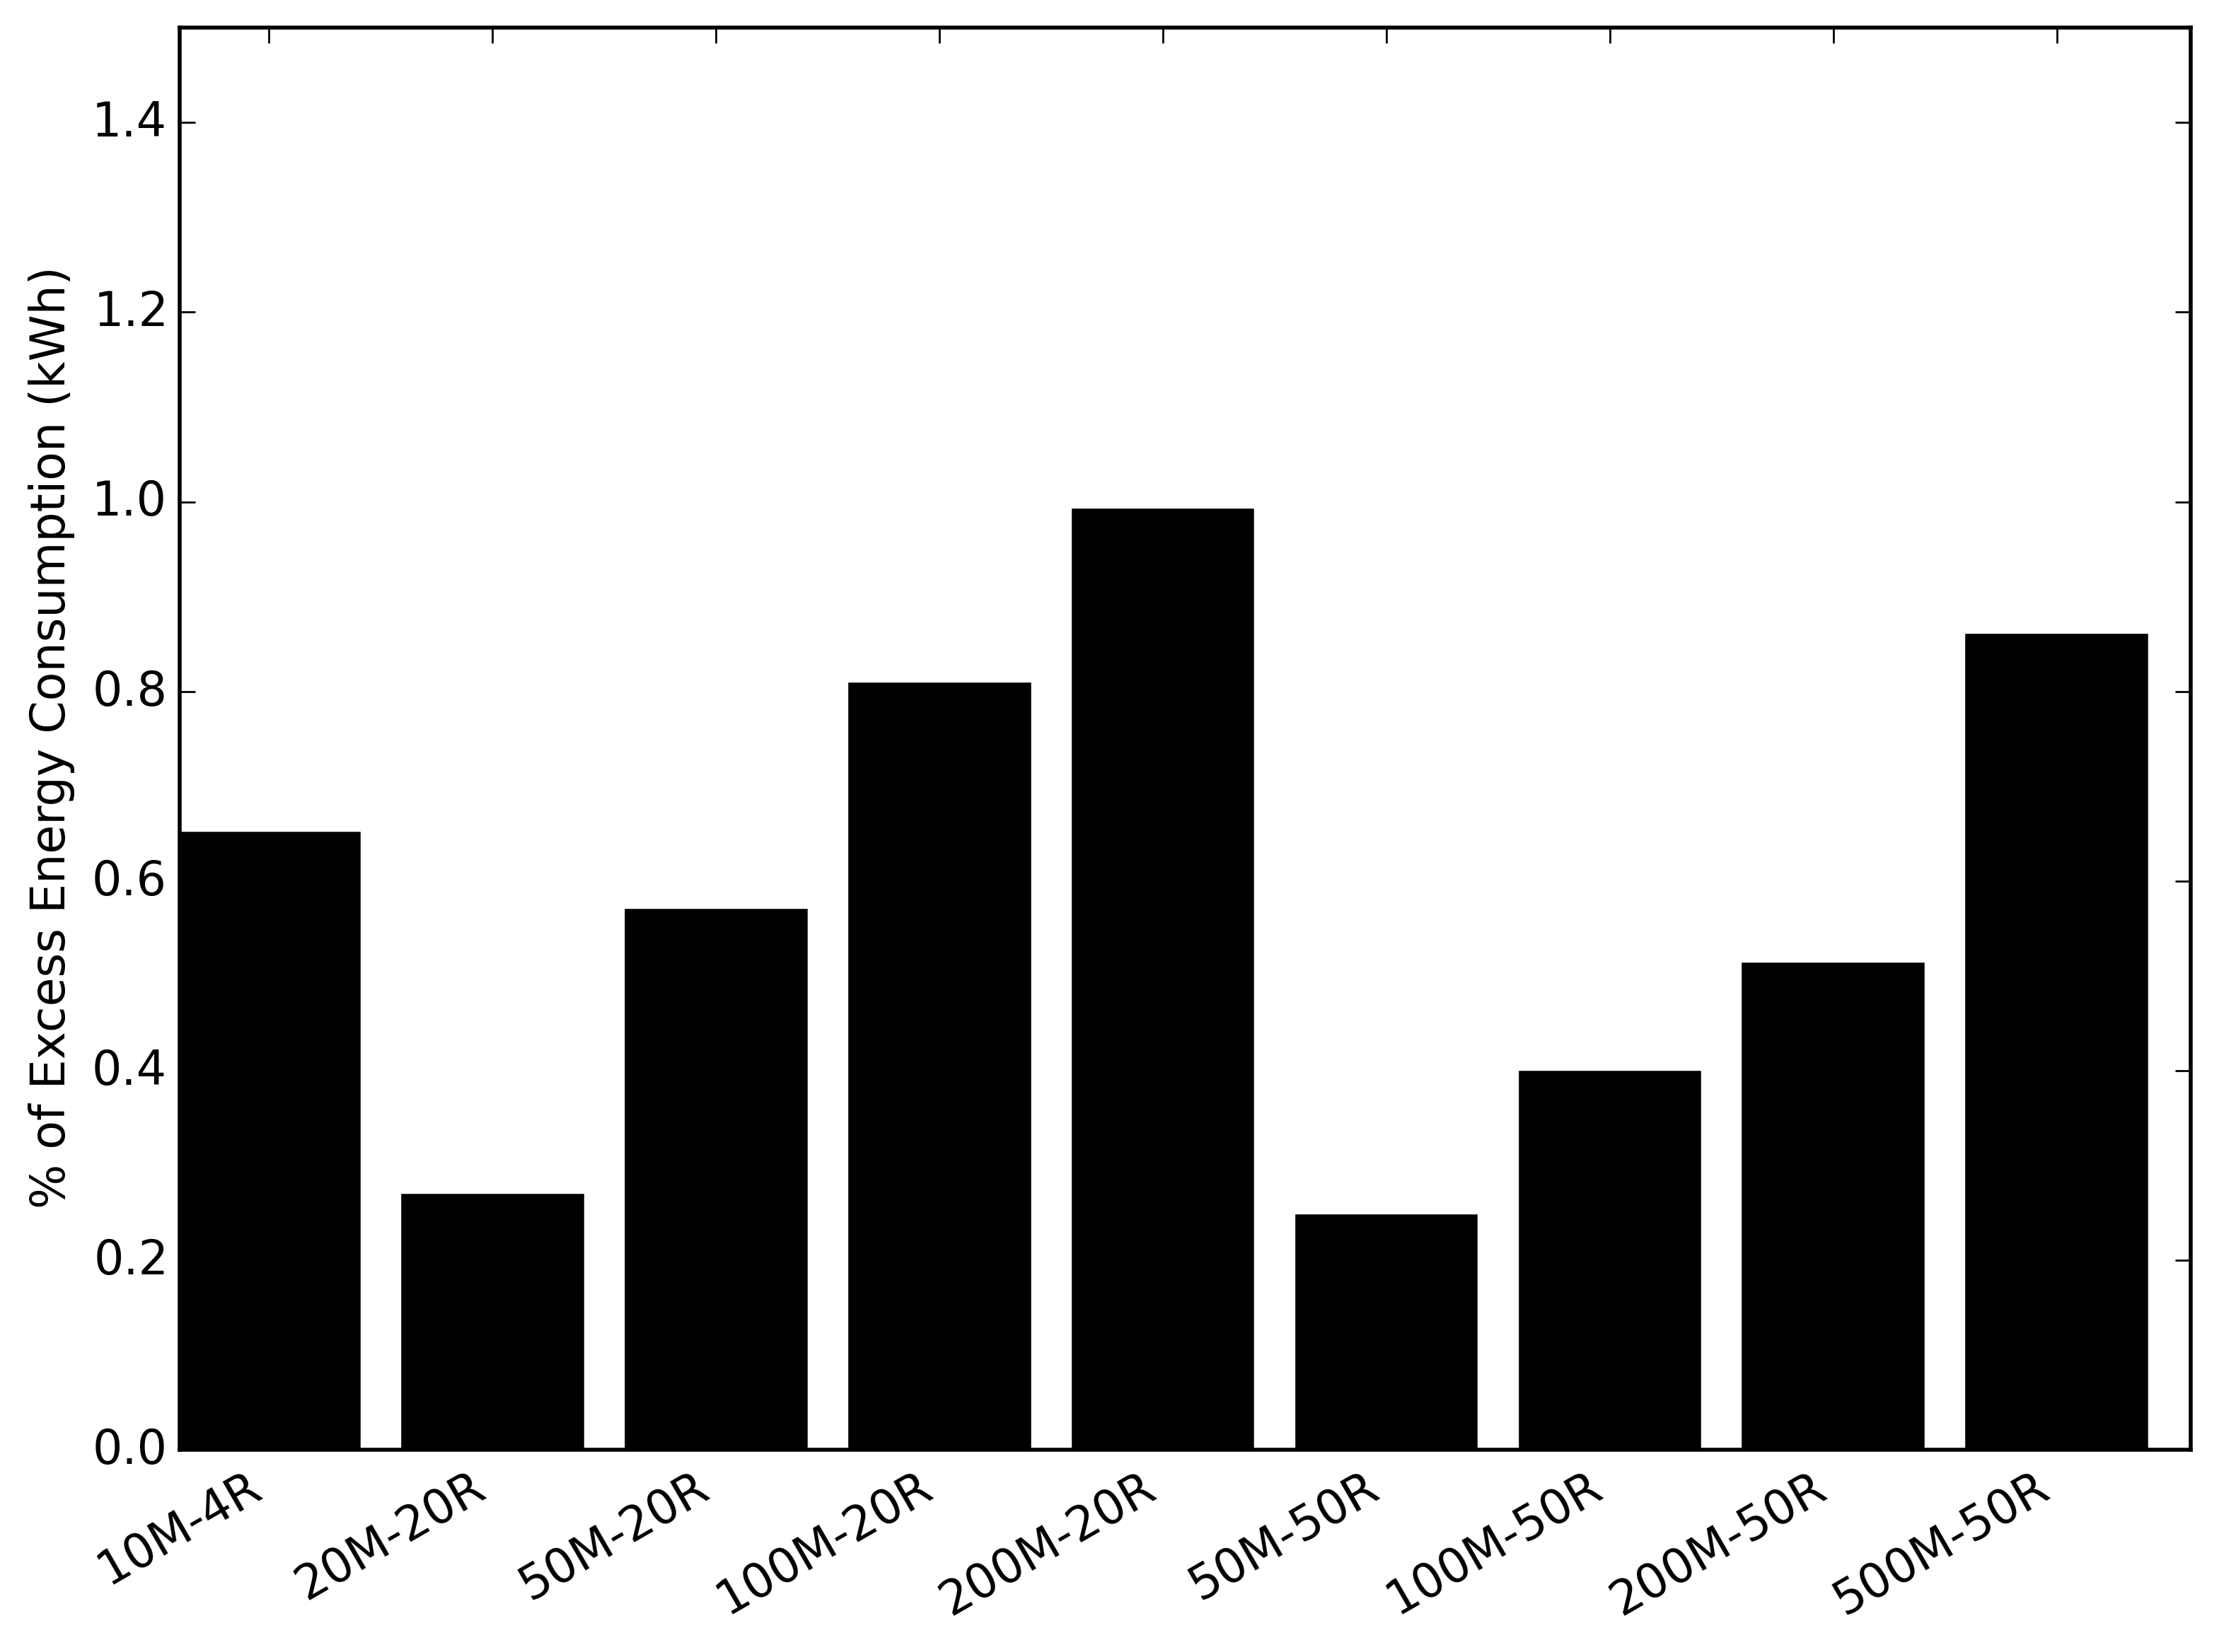
\includegraphics[width=.8\linewidth]{figs/perc_excess_energy_oracle_def_compile_mtd.png}
\end{tabular}
\caption{Online vs. offline scheduling}
\label{fig:oracle_vs}
\end{figure}

%0   1   1086.89   1054.6   32.29   3.06182438839
%0   2   1086.89   1046.84   40.05   3.82579954912
%0   3   1086.89   1034.17   52.72   5.09780790392
%0   4   1086.89   938.83   148.06   15.7706933098
%5   6   4934.22   4928.49   5.73   0.116262790429
%5   7   4934.22   4871.77   62.45   1.28187496536
%5   8   4934.22   4718.09   216.13   4.58087912693
%5   9   4934.22   4620.63   313.59   6.78673687354
%10   11   5197.34   5160.12   37.22   0.721301055014
%10   12   5197.34   5026.82   170.52   3.39220421658
%10   13   5197.34   4914.0   283.34   5.76597476597
%10   14   5197.34   4692.71   504.63   10.7534878567
%15   16   5497.76   5443.64   54.12   0.994187712633
%15   17   5497.76   5248.63   249.13   4.74657196259
%15   18   5497.76   5066.95   430.81   8.50235348681
%15   19   5497.76   4733.29   764.47   16.1509225084
%20   21   6258.15   6106.18   151.97   2.48879004549
%20   22   6258.15   5795.47   462.68   7.98347674994
%20   23   6258.15   5503.81   754.34   13.7057783608
%20   24   6258.15   4913.25   1344.9   27.3729201649
%25   26   12202.22   12150.95   51.27   0.421942317267
%25   27   12202.22   12033.22   169.0   1.40444536043
%25   28   12202.22   11927.74   274.48   2.30119033446
%25   29   12202.22   11629.3   572.92   4.92652180269
%30   31   12518.28   12475.19   43.09   0.345405560957
%30   32   12518.28   12268.26   250.02   2.03794181082
%30   33   12518.28   12082.84   435.44   3.6037885133
%30   34   12518.28   11774.85   743.43   6.31371100269
%35   36   13306.09   13160.57   145.52   1.10572718355
%35   37   13306.09   12858.53   447.56   3.48064669912
%35   38   13306.09   12563.96   742.13   5.90681600387
%35   39   13306.09   11919.53   1386.56   11.6326734359
%40   41   15801.01   15536.29   264.72   1.70388168604
%40   42   15801.01   14740.27   1060.74   7.19620468282
%40   43   15801.01   13782.34   2018.67   14.6467871203
%40   44   15801.01   12279.7   3521.31   28.6758634169
\begin{figure}[h]
\centering
\begin{tabular}{c}
  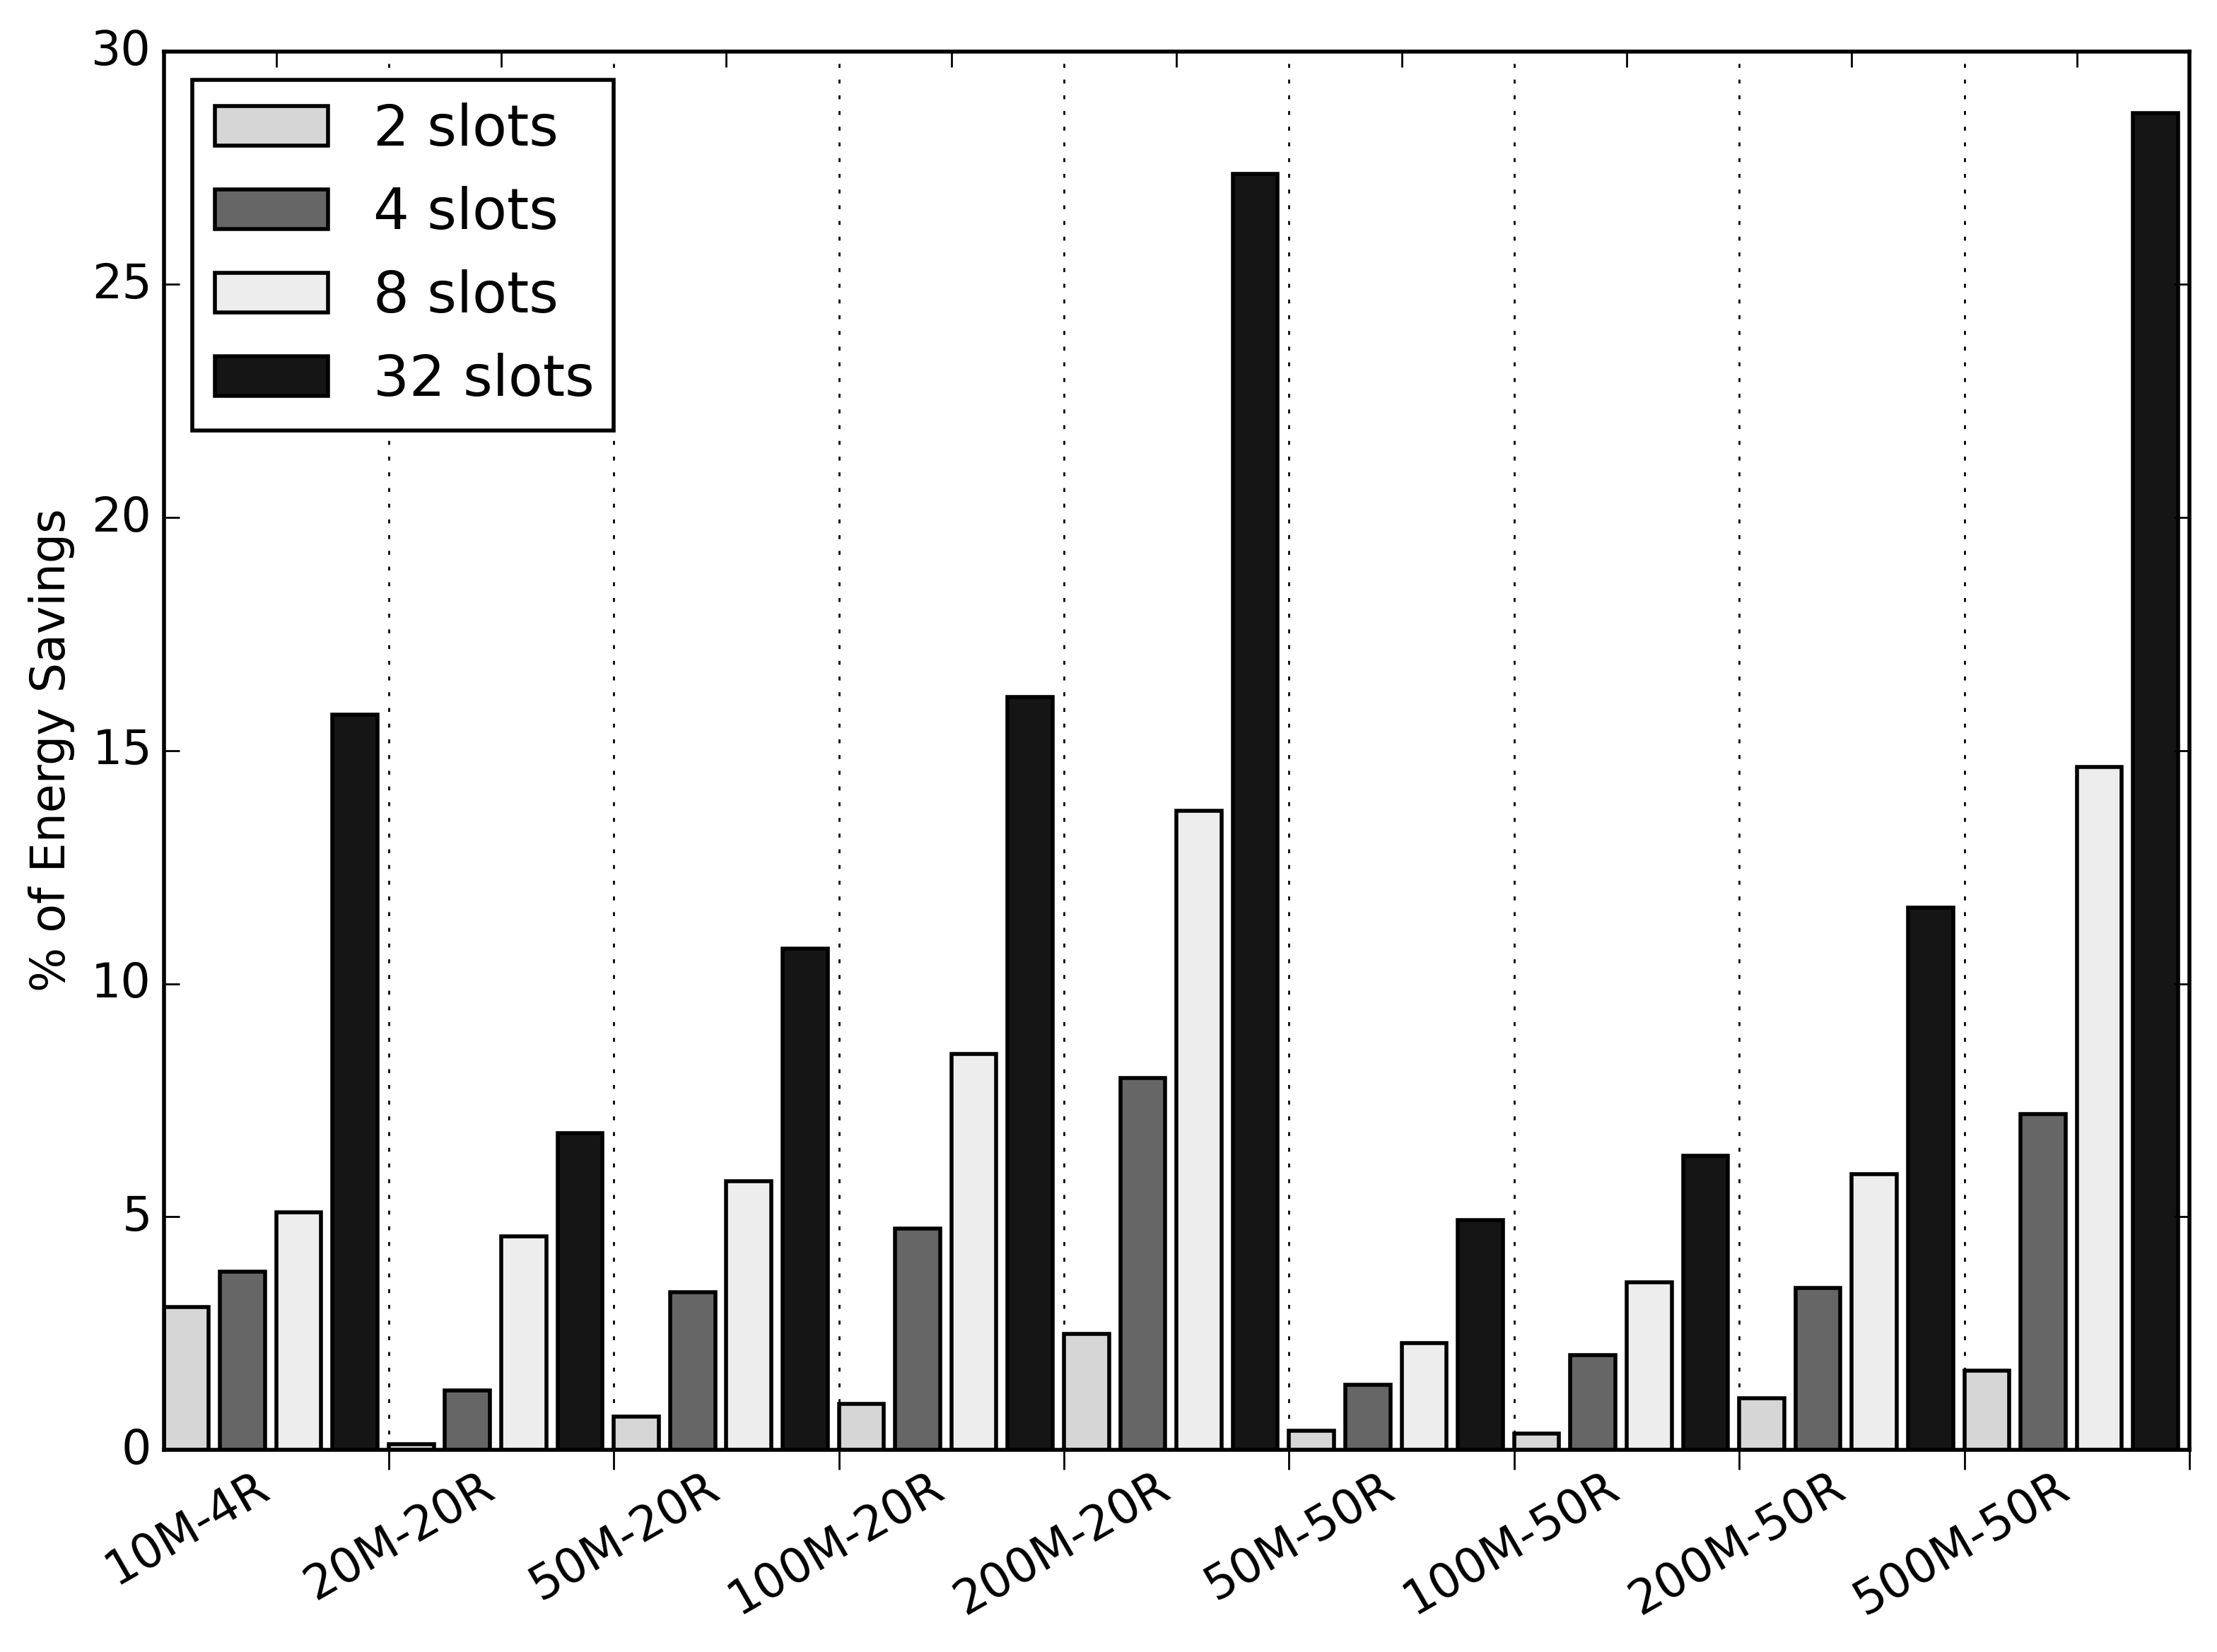
\includegraphics[width=0.8\linewidth]{figs/energy_tf_def_mtd_perc.png} 
\end{tabular}
\caption{Time flexibility vs. energy savings}
\label{fig:online_tf}
\end{figure}

The difference of solution quality, that is the excess consumption of the online scheduling as a percentage of the offline scheduling consumption, is shown in Fig.~\ref{fig:oracle_vs}. The results show that the offline solutions are merely 1\% better than the online solutions for tightly constrained problems (such as 200M-20R, 500M-50R). Note that in the online approach, at most 20 requests arrive in each online session and a maximum of 4 rooms are destroyed, thus the sub-problems formed are small enough for MIP to solve them to (near) optimality. The offline approach has many more meetings to deal with, but on the other hand, as problems become more constrained, it has more room to optimise than the greedy online approach. Altogether, even with a simple greedy approach, our online algorithm is able to perform effectively without prior knowledge of future requests. 

We also investigate the impact of energy savings with different time flexibility and request-to-start time gap. 
The amount of energy savings from meetings with 2 slots to 32 slots of permissible start time, as a percentage of the energy consumption incurred by meetings with strictly 1 permissible start time, is shown in Figure \ref{fig:online_tf}. We note that meetings with higher time flexibility achieve more energy savings than that of with lower time flexibility. The total savings can go up to 2.5\% with 2 flexible starting slots, and 28.7\% with 32 flexible starting slots. We also observe that, while a longer request-to-start time gap can lead to some savings on energy consumption, the influence of request-to-start time gap is relatively obvious when it comes to generating feasible solutions, which is covered in the next section.


\begin{figure}
\centering
\begin{tabular}{c}
  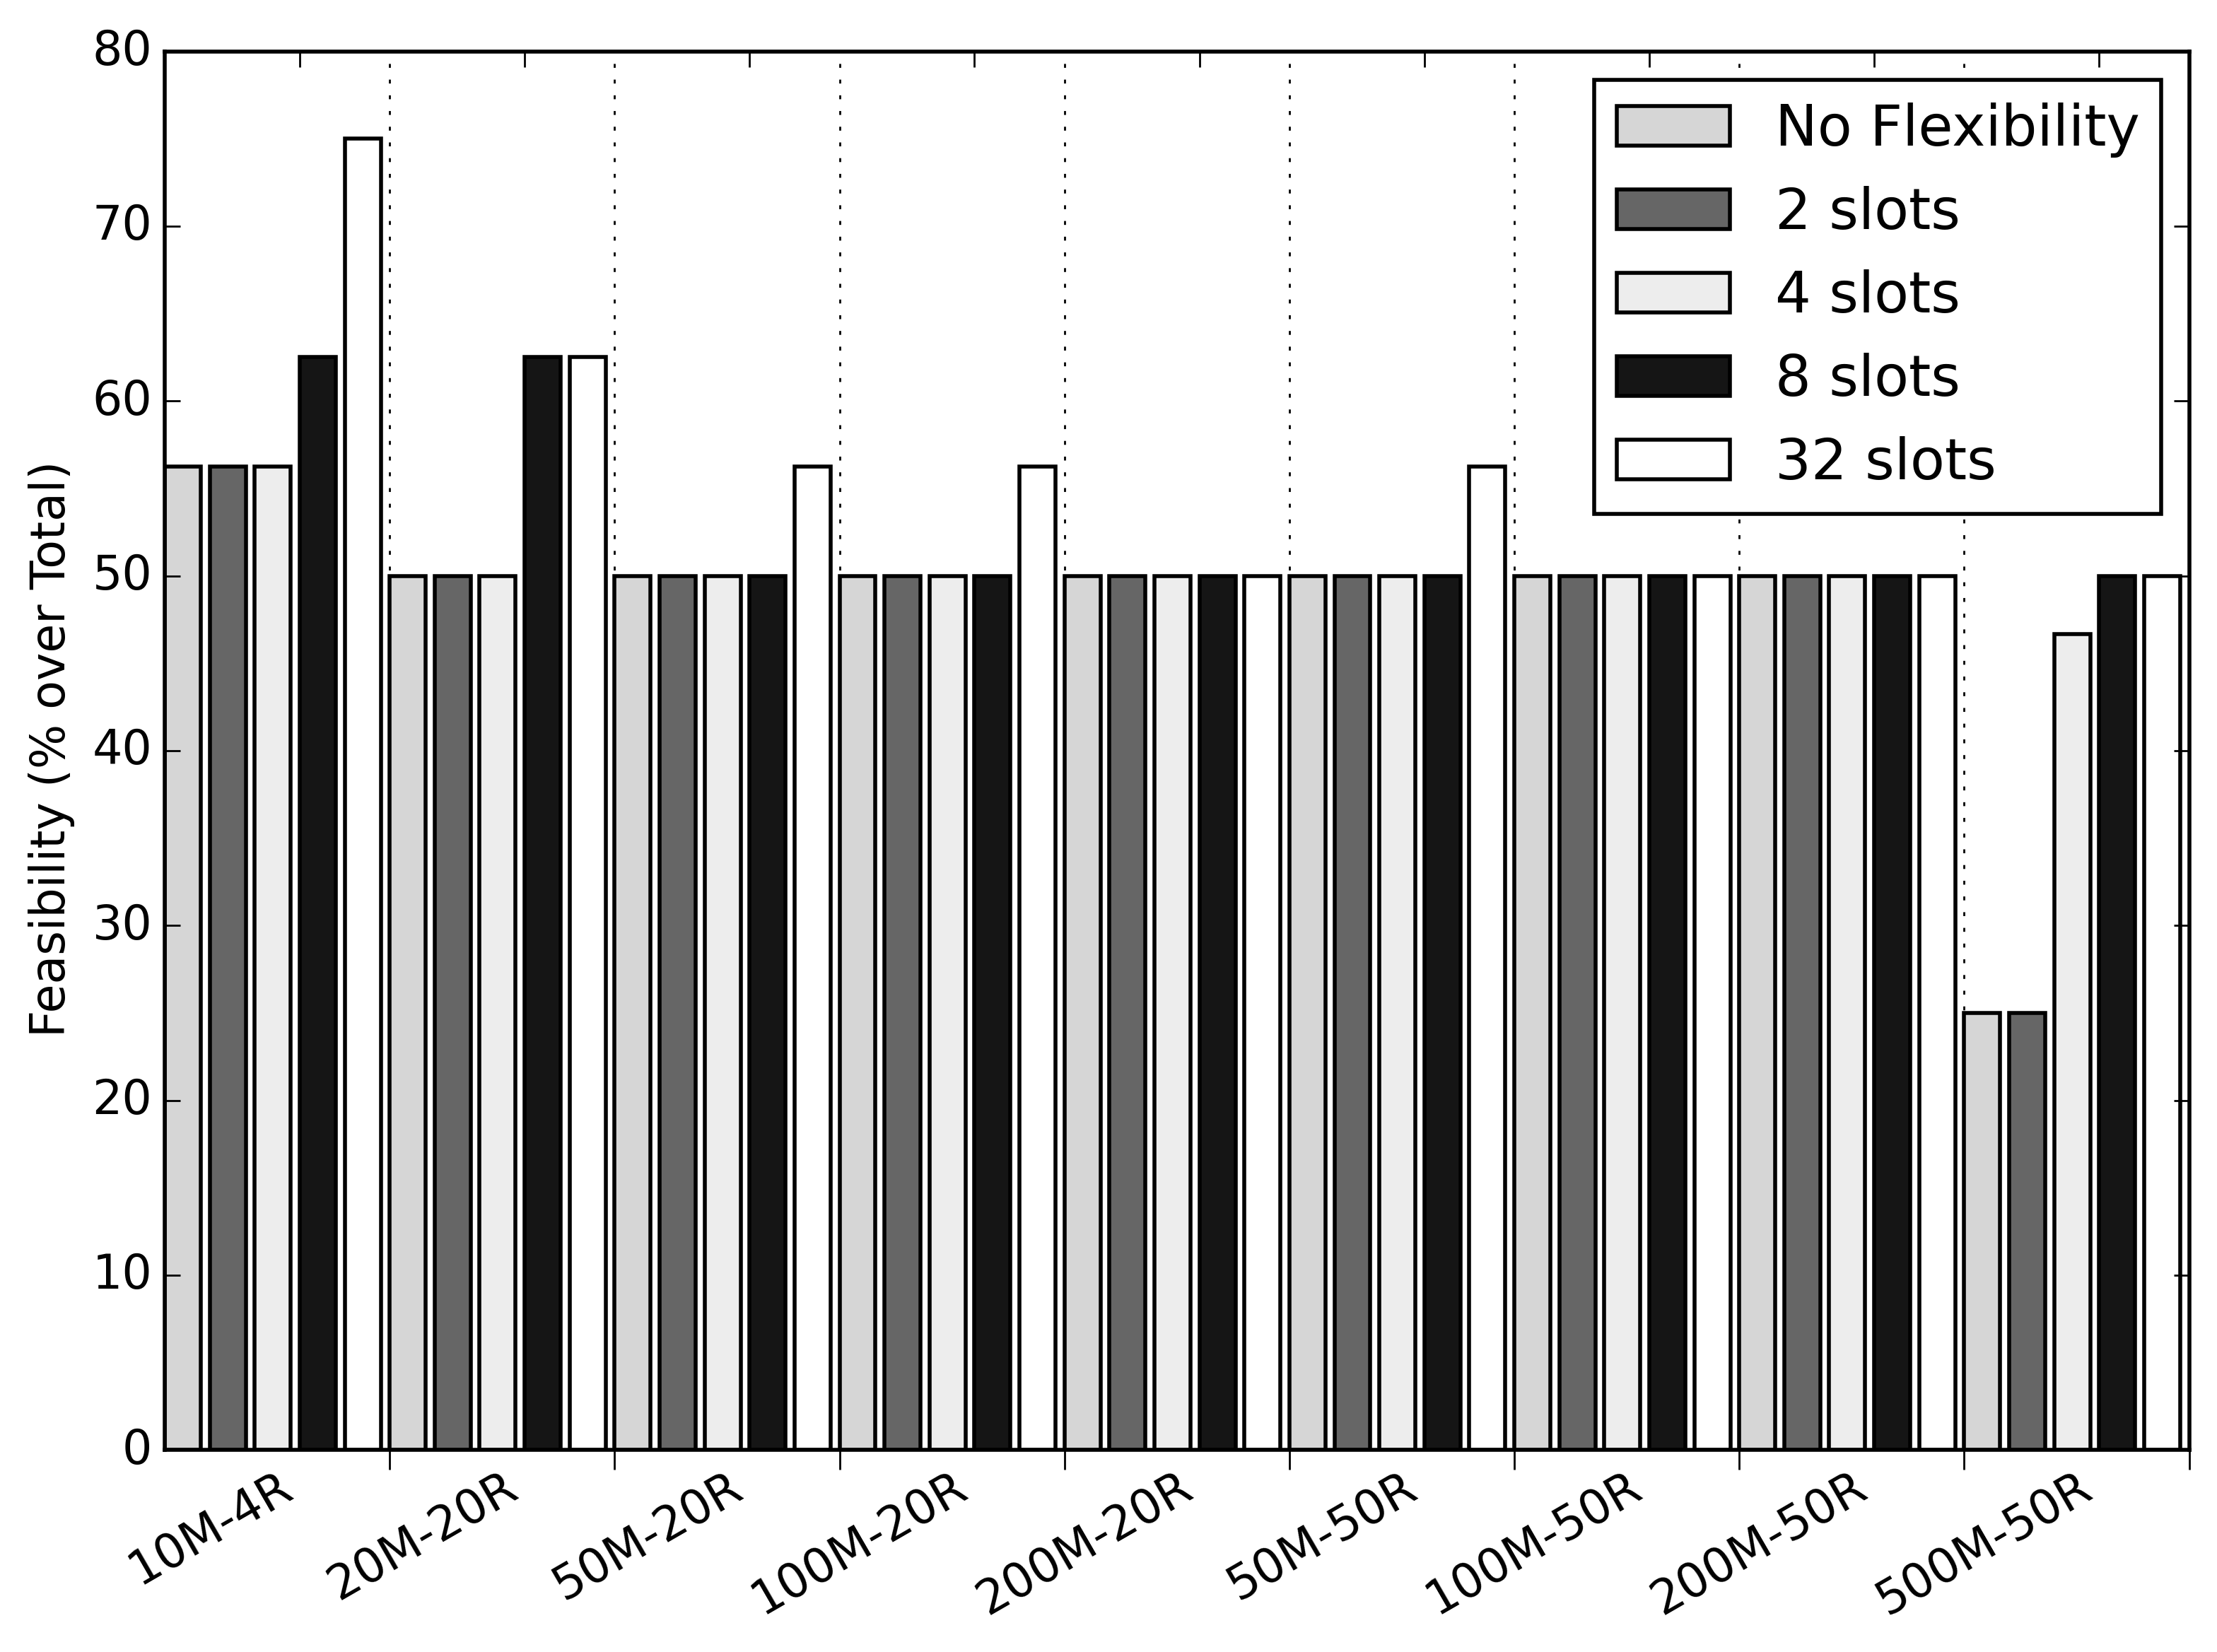
\includegraphics[width=0.8\linewidth]{figs/feasibility_tf_def_mtd.png} \\
(a) Time flexibility \\[6pt]
  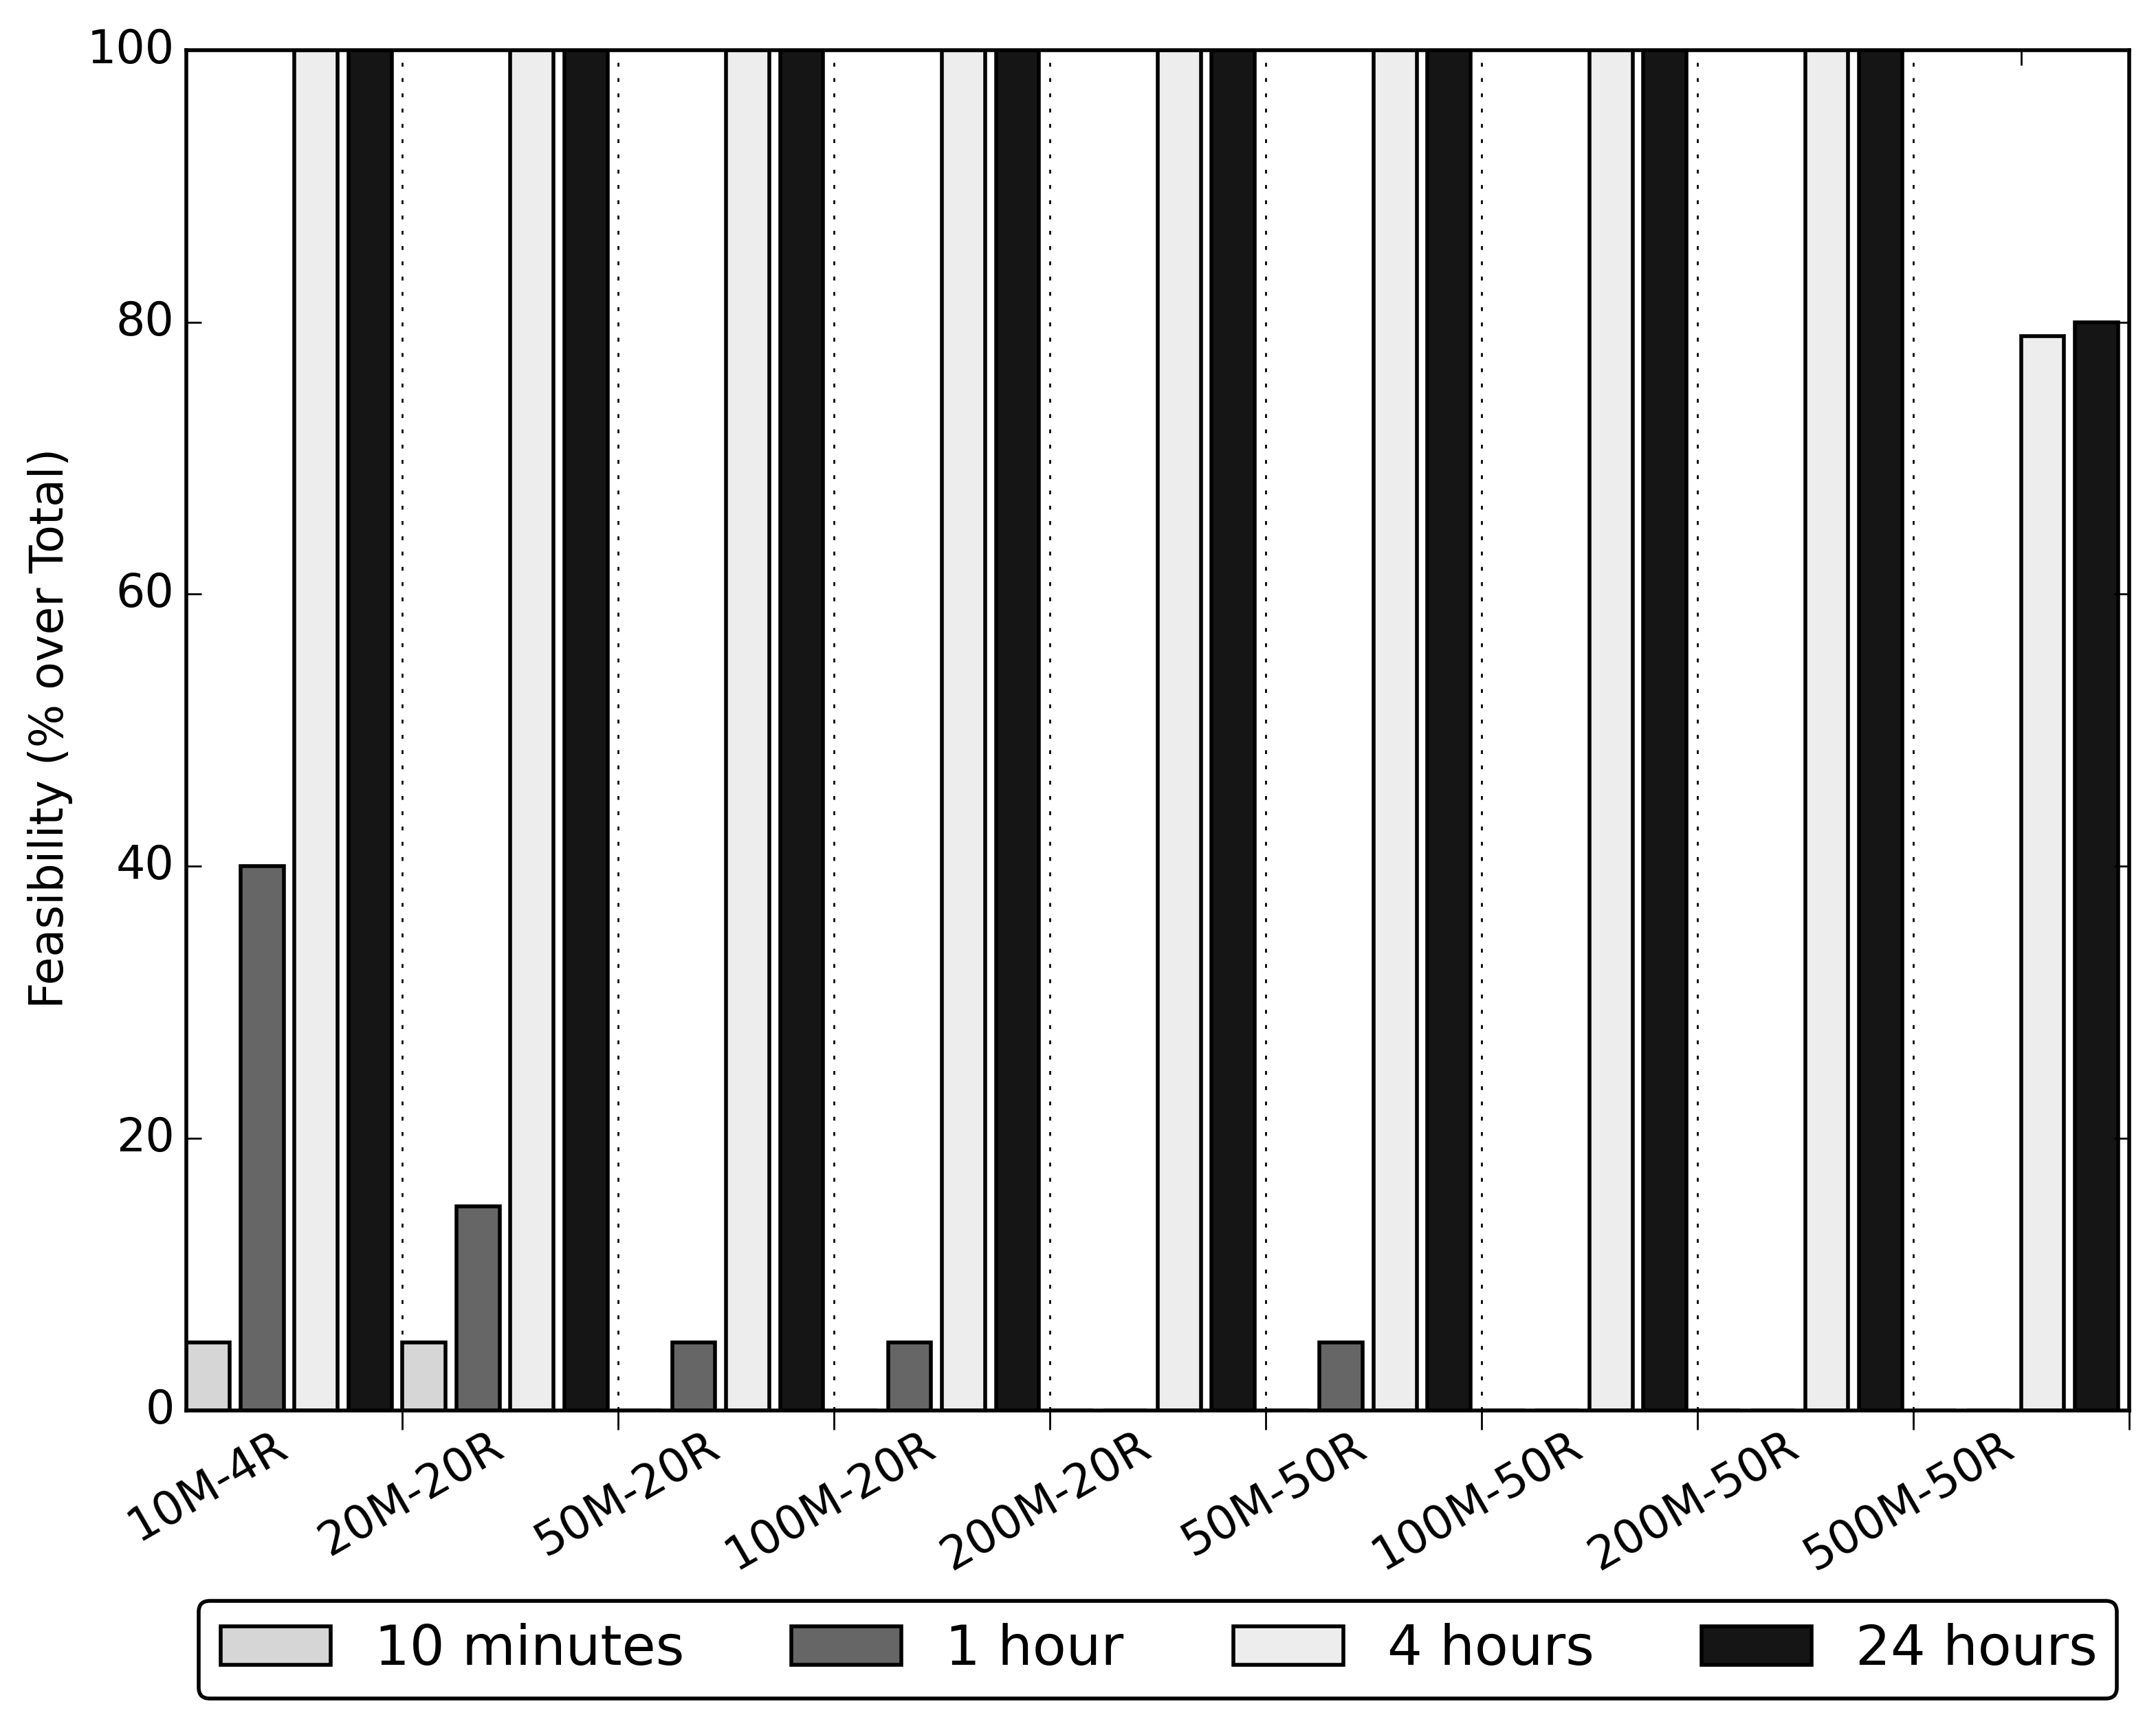
\includegraphics[width=0.8\linewidth]{figs/feasibility_cvs_def_mtd.png} \\
(b) Request-to-Start time gap \\[6pt]
\end{tabular}
\caption{Solution feasibility}
\label{fig:def_feas}
\end{figure}


\subsection{Model Feasibility}

%From the experiments, we notice two important properties that constraint the solution feasibility of our online solution. These properties are: (1) time flexibility, i.e. the number of possible starting slot for a meeting; and (2) request-to-start time gap, i.e the time gap between the request arrival time and its start time. 
From the experiments, we notice that time flexibility and request-to-start time gap constrain the solution feasibility of our online solution. In this section, we investigate further how different settings of these properties impact the feasibility performance of our model. Figure \ref{fig:def_feas} depicts the percentage of problem instances which are solvable, given different time flexibility and request-to-start time gap. 

In terms of time flexibility, Figure \ref{fig:def_feas}(a) shows that the number of problem instances which is solvable  does not vary a lot for problems with less than 4 possible starting slots. However, time flexibility impacts loosely constrained problems such as 10M-4R and tightly constrained problems such as 500M-50R. In these problems, more feasible solutions are generated with more time flexibility granted. 

Meanwhile, from Figure \ref{fig:def_feas}(b), we observe that the we fail to generate feasible solutions in most cases when the requests arrive less than 1 hour prior to the earliest possible activity start time. This infeasibility issue mainly happens at the initialization stage, where the initial schedule generation is decoupled from the initial HVAC control generation. In order to quickly generate an initial feasible schedule, activities are packed into the minimum number of rooms possible. However, the room temperatures may be too far from the temperature setpoints to obtain an initial feasible HVAC control reaching the designated occupied temperature at short notice. From these observations, we discover that fixing temperature setpoints between 21$^\circ$C to 23$^\circ$C is one of the root cause for these infeasibility issues. This motivates us to further investigate adaptive temperature setpoints control (see Chapter \ref{cha:atc}).

Apart from constrainedness imposed on temperature setpoints, the model also stumbles into infeasibility when the scheduler fails to schedule all requests due to the lack of feasible locations or time slots. There are existing techniques which can be introduced to overcome these issues, for example, by re-scheduling meetings at a different location or time slots. However it is out of the scope of this work and may be integrated in future. 
 

\section{Related Work} \label{sec:online:related_work}

Much of the existing literature on energy-oriented online scheduling focuses on workload scheduling in data center \citep{wang2009towards,kliazovich2013dens} and residential load control with respect to real-time electricity pricing \citep{mohsenian2010optimal,scott2013residential}. 

Existing works on energy-aware occupancy scheduling \citep{chai2014minimizing,lim2015hvac,lim2015large,majumdar2016characterising,majumdar2012energy,pan2013minimizing,pan2012thermal} focus on offline scheduling, and assume that all activities to schedule and other parameters such as the weather forecast are known in advance.

The work that is closest to ours is that presented by \cite{kwak2013tesla}. They formulate their scheduling problem as a two-stage stochastic model with sample average approximation (SAA) method \citep{pagnoncelli2009sample}. The first stage minimises the energy consumption when new meeting requests are scheduled, together with the expected energy consumption that will be realized by future meeting requests. The second stage considers multiple sample sets of future meetings based on the likelihood of \emph{\textsl{k}} future requests that will arrive. They create 50 sample sets of future requests for every session. Each sample set possesses a likelihood that a particular set of future meeting requests will be realized. They derive this likelihood value based on a probability distribution over the possible range of total requests arrived per day at the USC library. 
The benefit of this stochastic modeling technique is that, if the future meetings are accurately anticipated, then it may reduce the energy consumption more than our greedy-based approach.
On the other hand, the drawback of this approach is that, if the future meetings turn out not being held, energy can be wasted by scheduling real meetings in rooms that are not energy-efficient simply because the other rooms are presumably occupied. 
In contrast, our greedy-based scheduling algorithm is computationally efficient by considering only real meeting requests, and is less complex to implement compare to their two-stage stochastic model. While we assume no prior knowledge of future meetings, the quality of our solution is within 1\% of that of the clairvoyant solution. This is achieved by the fact that our HVAC control is continuously optimised while the schedule is fixed. When a new request arrives, the scheduler identifies the best time and location, as well as the HVAC control settings that are optimised for both pre-scheduled and new meetings. In this scenario, the stochastic approach is over-kill compared to our greedy approach.

%% Their work calculates energy consumption based on historical data and exploits flexibility in the time and location at which a meeting can take place. However, it does not optimise HVAC control, nor does it take thermal comfort flexibility into account. 
%% Our results show that combining meeting scheduling with HVAC control, and enabling adaptive temperature control based on occupant thermal comfort flexibility, significantly impacts energy savings.

\cite{kwak2013tesla} have also considered deadline flexibility, where a deadline by which the time and location for the meeting should be notified to the user can be flexibly set. This allows the scheduler to reschedule existing requests when a more energy-efficient schedule can be found with the arrival of new meeting requests. However, in their experiments, they have shown that the advantage of having deadline flexibility is insignificant, instead time flexibility and location flexibility are able to produce more pronounced energy savings.
Whilst we assume zero deadline flexibility based on the fact that majority of the users would expect an immediate feedback upon submitting a meeting request, it might be interesting to find out if our joint model makes a difference with this feature being integrated in the future. 

%\cite{mady2011stochastic} consider a stochastic building occupancy model to improve on the energy efficiency while minimising expected discomfort.

\section{Conclusion and Future Work} \label{sec:online:conclusion}

%http://research.microsoft.com/en-us/um/people/sebubeck/BubeckLectureNotes.pdf

%Specifically, we present the online mechanism that adopt greedy-based scheduling method but revising the HVAC control strategy upon receiving new requests.

% a joint HVAC control and occupancy scheduling model which handles dynamically arriving scheduling requests


In this chapter we developed an online scheduling model for joint HVAC control and occupancy scheduling. Leveraging an explicit model of building occupancy-based HVAC control, our model adopts a greedy approach to schedule dynamically arriving requests to take place at locations and times that are favorable from energy standpoint. Our experiments show that, even without prior knowledge of future requests, our model is able to produce energy-efficient schedules which are less than 1\% away from the clairvoyant solution. Overall, the solution quality, in terms of energy savings and solution feasibility, improves as the request-to-start time gap and the time window flexibility increase. 

There are existing works that consider re-scheduling or re-locating meetings using multi-agent systems \citep{kwak2014building,klein2012coordinating}. However, they adopt a Markov decision process that suffers from scalability issues. We are interested in exploring efficient techniques that fit in our joint model to re-schedule meetings considering users' deadline flexibility and request cancellations. 

We are particularly interested in exploring alternative online scheduling algorithms, with the aim of further improving the solution quality under the circumstances when a lot of online requests arrive within a short notice. In the next chapter, we present one alternative which improves on the solution quality by introducing the concept of adaptive temperature control.

%Regarding uncertainty: for the purpose of generating good meeting schedules (as opposed to precise HVAC control plans), we speculate that using average seasonal temperatures (say month by month) as the forecast gives good results. This is because seasonal temperature variations are significant whilst within a few weeks, temperature patterns tend to be quite similar. However, our future work agenda includes testing this hypothesis and handling uncertainty using stochastic programming at two different scales: 
%1. to generate, days in advance, schedules with optimal expected costs over sampled scenarios for external temperature. In that case, there is one set of meeting scheduling decision variables, but the various scenarios give rise to different HVAC control decisions. 
%2. to re-optimise HVAC control, minutes to a day in advance for a given meeting schedule. In that case, we plan to use online stochastic programming over a receding horizon. This is similar to our work on residential energy management see [Scott et. al, CP 2013]. 

